\documentclass[a4paper,twoside,11pt]{book}

% ----------------------------------------------------------------
% PAQUETES ESENCIALES
% ----------------------------------------------------------------
\usepackage{listings}           % Para mostrar código fuente
\usepackage[utf8]{inputenc}     % Codificación de caracteres (tildes, ñ...)
\usepackage[spanish]{babel}     % Idioma español (separación silábica, fechas...)
\usepackage[T1]{fontenc}        % Codificación de fuente correcta para español
\usepackage{amsmath}   % Fórmulas matemáticas avanzadas
\usepackage{amssymb}   % Símbolos matemáticos (\mathbb, etc.)
\usepackage{pgfgantt}   % Diagramas de Gantt
\usepackage{eurosym}    % Símbolo del euro (\euro)
\usetikzlibrary{arrows.meta, positioning, fit, backgrounds, shapes.geometric}  % Diagramas de arquitectura y ETL (Cap. 3)

% ----------------------------------------------------------------
% MATEMÁTICAS Y TABLAS
% ----------------------------------------------------------------
\decimalpoint
\usepackage{dcolumn}
\newcolumntype{.}{D{.}{\esperiod}{-1}}
\makeatletter
\addto\shorthandsspanish{\let\esperiod\es@period@code}
\makeatother

% ----------------------------------------------------------------
% LAYOUT Y MÁRGENES
% ----------------------------------------------------------------
\usepackage{geometry}
\geometry{
  a4paper,
  top=3cm,
  bottom=3cm,
  inner=3.5cm,  % Margen interior (lomo) — se alterna izq/der según la página
  outer=2.5cm   % Margen exterior — siempre al borde de la hoja
}

% ----------------------------------------------------------------
% CABECERAS Y PIES DE PÁGINA
% ----------------------------------------------------------------
\RequirePackage{verbatim}
\usepackage{fancyhdr}
\usepackage{graphicx}
\usepackage{afterpage}
\usepackage{longtable}

% ----------------------------------------------------------------
% ENLACES E HIPERVÍNCULOS (sin bordes visibles)
% ----------------------------------------------------------------
\usepackage[hidelinks]{hyperref}

% ----------------------------------------------------------------
% INFORMACIÓN DEL DOCUMENTO (cámbiala cuando quieras)
% ----------------------------------------------------------------
\newcommand{\myTitle}{Sistema de Cálculo de Rutas Seguras en Entornos Urbanos Mediante Análisis Espacial\xspace}
\newcommand{\myDegree}{Grado en Ingeniería Informática\xspace}
\newcommand{\myName}{Soto Zaragoza, Adriana\xspace}
\newcommand{\myEmail}{adrianasoto@correo.ugr.es\xspace}
\newcommand{\myProf}{Samos Jiménez, José\xspace}
\newcommand{\myOtherProf}{\xspace}
\newcommand{\myFaculty}{Escuela Técnica Superior de Ingenierías Informática y de
Telecomunicación\xspace}
\newcommand{\myFacultyShort}{E.T.S. de Ingenierías Informática y de
Telecomunicación\xspace}
\newcommand{\myDepartment}{Departamento de Lenguajes y Sistemas Informáticos\xspace}
\newcommand{\myUni}{\protect{Universidad de Granada}\xspace}
\newcommand{\myLocation}{Granada\xspace}
\newcommand{\myTime}{Septiembre de 2026\xspace}
\newcommand{\myVersion}{Versión 1.0\xspace}

% Metadatos del PDF (visibles en "Propiedades del documento")
\hypersetup{
  pdfauthor   = {Adriana Soto Zaragoza},
  pdftitle    = {Sistema de Cálculo de Rutas Seguras en Entornos Urbanos},
  pdfsubject  = {Trabajo Fin de Grado - Ingeniería Informática - UGR},
  pdfkeywords = {rutas seguras, SIG, PostGIS, pgRouting, Madrid, movilidad urbana},
  pdfcreator  = {LaTeX},
  pdfproducer = {pdflatex}
}

% ----------------------------------------------------------------
% OTROS PAQUETES ÚTILES
% ----------------------------------------------------------------
\usepackage{url}
\usepackage{colortbl}
\usepackage[stable]{footmisc}   % Notas al pie estables
\usepackage{pgfgantt}           % Diagramas de Gantt
\usepackage{eurosym}            % Símbolo del euro (\euro)

% ----------------------------------------------------------------
% CONFIGURACIÓN DE CABECERAS (fancyhdr)
% ----------------------------------------------------------------
\setlength{\headheight}{14pt}

\pagestyle{fancy}
\fancyhf{}  % Limpia cabecera y pie por defecto

% Documento a doble cara (twoside):
% LO = Left Odd  (izquierda en páginas impares)
% RE = Right Even (derecha en páginas pares)
% RO = Right Odd  (derecha en páginas impares)
% LE = Left Even  (izquierda en páginas pares)
\fancyhead[LO]{\small\leftmark}             % Capítulo en páginas impares (izq.)
\fancyhead[RE]{\small\rightmark}            % Sección en páginas pares (der.)
\fancyhead[RO,LE]{\small\textbf{\thepage}} % Nº página siempre al exterior
\fancyfoot{}  % Sin pie de página

% Grosor de la línea bajo la cabecera
\renewcommand{\headrulewidth}{0.4pt}

% Formato del nombre de capítulo y sección en la cabecera
% (\@chapapp es "Capítulo" en el cuerpo y "Apéndice" tras \appendix)
\makeatletter
\renewcommand{\chaptermark}[1]{\markboth{\@chapapp\ \thechapter.\ #1}{}}
\makeatother
\renewcommand{\sectionmark}[1]{\markright{\thesection.\ #1}}

% ----------------------------------------------------------------
% COMANDOS DE APOYO
% ----------------------------------------------------------------
\newcommand{\HRule}{\rule{\linewidth}{0.5mm}}

% Entornos para teoremas, ejemplos y definiciones (útiles en cap. técnicos)
\newtheorem{teorema}{Teorema}[chapter]
\newtheorem{ejemplo}{Ejemplo}[chapter]
\newtheorem{definicion}{Definición}[chapter]

% ----------------------------------------------------------------
% CONFIGURACIÓN DE BLOQUES DE CÓDIGO (listings)
% Así se verá el código SQL, Python, etc. en los anexos
% ----------------------------------------------------------------
\usepackage{xcolor}
\definecolor{colorFondo}{gray}{.97}
\definecolor{colorComentario}{gray}{.45}

\lstset{
  frame=single,
  framerule=0.5pt,
  aboveskip=0.5cm,
  backgroundcolor=\color{colorFondo},
  stringstyle=\ttfamily,
  showstringspaces=false,
  basicstyle=\small\ttfamily,
  commentstyle=\color{colorComentario}\itshape,
  keywordstyle=\bfseries,
  numbers=left,
  numbersep=8pt,
  numberstyle=\tiny\color{gray},
  breaklines=true,
  captionpos=b,
  extendedchars=true,
  literate=
    {á}{{\'a}}1 {é}{{\'e}}1 {í}{{\'i}}1 {ó}{{\'o}}1 {ú}{{\'u}}1
    {Á}{{\'A}}1 {É}{{\'E}}1 {Í}{{\'I}}1 {Ó}{{\'O}}1 {Ú}{{\'U}}1
    {ñ}{{\~n}}1 {Ñ}{{\~N}}1 {ü}{{\"u}}1 {¿}{{?`}}1 {¡}{{!`}}1
}

% Estilo específico para SQL (útil para las consultas PostGIS/pgRouting)
\lstdefinestyle{SQL}{
  language=SQL,
  morekeywords={ST_Distance, ST_Buffer, pgr_dijkstra, geography, geometry}
}

% Estilo para Python (útil para los scripts ETL)
\lstdefinestyle{Python}{
  language=Python
}

% ----------------------------------------------------------------
% PÁGINAS EN BLANCO SIN CABECERA
% ----------------------------------------------------------------
\makeatletter
\def\clearpage{%
  \ifvmode
    \ifnum \@dbltopnum =\m@ne
      \ifdim \pagetotal <\topskip
        \hbox{}
      \fi
    \fi
  \fi
  \newpage
  \thispagestyle{empty}
  \write\m@ne{}
  \vbox{}
  \penalty -\@Mi
}
\makeatother

\usepackage{pdfpages}

% ================================================================
% INICIO DEL DOCUMENTO
% ================================================================
\begin{document}

% ----------------------------------------------------------------
% PÁGINAS PRELIMINARES (portada, declaración, resumen, etc.)
% Estas páginas NO llevan numeración ni cabecera
% ----------------------------------------------------------------
\begin{titlepage}
	
	
	\newlength{\centeroffset}
	\setlength{\centeroffset}{-0.5\oddsidemargin}
	\addtolength{\centeroffset}{0.5\evensidemargin}
	\thispagestyle{empty}
	
	\noindent\hspace*{\centeroffset}\begin{minipage}{\textwidth}
		
		\centering
		
\includegraphics[width=0.9\textwidth]{imagenes/logo_ugr.jpg}\\[1.4cm]
		
		\textsc{ \Large TRABAJO FIN DE GRADO\\[0.2cm]}
		\textsc{ GRADO EN INGENIERÍA INFORMÁTICA}\\[1cm]
		% Upper part of the page
		% 
		% Title
		{\Large\bfseries Sistema de Cálculo de Rutas Seguras en Entornos Urbanos Mediante Análisis Espacial\\
		}
		\noindent\rule[-1ex]{\textwidth}{3pt}\\[3.5ex]
		{\large\bfseries Integración de factores de riesgo y datos abiertos en la ciudad de Madrid}
	\end{minipage}
	
	\vspace{2.5cm}
	\noindent\hspace*{\centeroffset}\begin{minipage}{\textwidth}
		\centering
		
		\textbf{Autor}\\ {Soto Zaragoza, Adriana}\\[2.5ex]
		\textbf{Director}\\
		{Samos Jiménez. José}\\[2cm]
		
\includegraphics[width=0.3\textwidth]{imagenes/etsiit_logo.png}\\[0.1cm]
		\textsc{Escuela Técnica Superior de Ingenierías Informática y de Telecomunicación}\\
		\textsc{---}\\
		Granada, Junio de 2026
	\end{minipage}
	%\addtolength{\textwidth}{\centeroffset}
	%\vspace{\stretch{2}}
\end{titlepage}



\chapter*{}
%\thispagestyle{empty}
%\cleardoublepage

%\thispagestyle{empty}

\begin{titlepage}
 
 
\setlength{\centeroffset}{-0.5\oddsidemargin}
\addtolength{\centeroffset}{0.5\evensidemargin}
\thispagestyle{empty}

\noindent\hspace*{\centeroffset}\begin{minipage}{\textwidth}

\centering
%
\includegraphics[width=0.9\textwidth]{imagenes/logo_ugr.jpg}\\[1.4cm]

%\textsc{ \Large PROYECTO FIN DE CARRERA\\[0.2cm]}
%\textsc{ GRADO EN INGENIERÍA INFORMÁTICA}\\[1cm]
% Upper part of the page


\vspace{3.3cm}

%si el proyecto tiene logo poner aquí
% 
\includegraphics{imagenes/logo.png} 
\vspace{0.5cm}

% Title

{\Huge\bfseries Sistema de Cálculo de Rutas Seguras en Entornos Urbanos Mediante Análisis Espacial\\
}
\noindent\rule[-1ex]{\textwidth}{3pt}\\[3.5ex]
{\large\bfseries Integración de factores de riesgo y datos abiertos en la ciudad de Madrid.}\\[4cm]
\end{minipage}

\vspace{2.5cm}
\noindent\hspace*{\centeroffset}\begin{minipage}{\textwidth}
\centering

\textbf{Autor}\\ {Soto Zaragoza, Adriana}\\[2.5ex]
\textbf{Director}\\
{Samos Jiménez, José}\\[2cm]
%
\includegraphics[width=0.15\textwidth]{imagenes/tstc.png}\\[0.1cm]
%\textsc{Departamento de Lenguajes y Sistemas Informáticos}\\
%\textsc{---}\\
%Granada, mes de 2026
\end{minipage}
%\addtolength{\textwidth}{\centeroffset}
\vspace{\stretch{2}}

 
\end{titlepage}






\cleardoublepage
\thispagestyle{empty}

\begin{center}
{\large\bfseries Sistema de Cálculo de Rutas Seguras en Entornos Urbanos Mediante Análisis Espacial: Integración de factores de riesgo y datos abiertos en la ciudad de Madrid}\\
\end{center}
\begin{center}
Adriana Soto Zaragoza\\
\end{center}

\noindent{\textbf{Palabras clave}: rutas seguras, Sistemas de Información Geográfica, PostGIS, pgRouting, seguridad peatonal, análisis espacial, datos abiertos, Madrid}\\

\vspace{0.7cm}
\noindent{\textbf{Resumen}}\\

La movilidad peatonal urbana manifiesta ciertos riesgos que los sistemas de navegación convencionales ignoran cuando se prioriza principalmente la distancia o el tiempo de desplazamiento. Este Trabajo Fin de Grado presenta el diseño y desarrollo de un sistema de cálculo de rutas seguras para peatones en la ciudad de Madrid, basado en el análisis espacial de datos abiertos georreferenciados. El sistema integra indicadores de riesgo urbano obtenidos del portal de Datos Abiertos y del Geoportal del Ayuntamiento de Madrid, como el servicio de iluminación pública de la ciudad, un índice de vulnerabilidad territorial por distritos y la accidentalidad con víctimas peatonales. Mediante un proceso ETL, los datos se han incorporado a una base de datos espacial implementada en PostgreSQL/PostGIS donde se modela la red peatonal a través de un grafo ponderado. Los pesos de las aristas reflejan el nivel de riesgo de cada segmento de calle según los indicadores definidos. El motor de enrutamiento pgRouting calcula a partir de este grafo la ruta que minimiza la exposición a dicho riesgo. El sistema se expone a través de un prototipo de visor cartográfico web desarrollado con Leaflet, que permite comparar la ruta segura con la ruta más corta convencional.
\cleardoublepage


\thispagestyle{empty}

\begin{center}
{\large\bfseries A Safe Routing System for Urban Environments via Spatial Analysis: Integrating Risk Factors and Open Data in Madrid}\\
\end{center}
\begin{center}
Adriana Soto Zaragoza\\
\end{center}

%\vspace{0.7cm}
\noindent{\textbf{Keywords}: safe routing, Geographic Information Systems, PostGIS, pgRouting, pedestrian safety, spatial analysis, open data, Madrid}\\

\vspace{0.7cm}
\noindent{\textbf{Abstract}}\\

Pedestrian mobility in urban environments entails specific risks that conventional navigation systems overlook when prioritising distance or travel time. This Bachelor's Thesis presents the design and development of a safe route calculation system for pedestrians in the city of Madrid, based on spatial analysis of georeferenced open data. The system integrates urban risk indicators such as public street lighting coverage, a district-level territorial vulnerability index, and pedestrian traffic accident records; all sourced from the Madrid City Council Open Data portal and Geoportal. Through an ETL pipeline, these datasets are processed and loaded into a spatial database built on PostgreSQL/PostGIS, where the pedestrian network is modelled as a weighted graph. Edge weights reflect the risk level of each street segment according to the defined indicators. Using this graph, the pgRouting extension computes the route that minimises risk exposure. The system is implemented as a web mapping prototype developed with Leaflet, enabling users to compare the safe route against the conventional shortest path.

\chapter*{}
\thispagestyle{empty}

\noindent\rule[-1ex]{\textwidth}{2pt}\\[4.5ex]

Yo, \textbf{Adriana Soto Zaragoza}, alumna de la titulación Ingeniería Informática de la \textbf{Escuela Técnica Superior
de Ingenierías Informática y de Telecomunicación de la Universidad de Granada}, con DNI 77244926R, autorizo la
ubicación de la siguiente copia de mi Trabajo Fin de Grado en la biblioteca del centro para que pueda ser
consultada por las personas que lo deseen.

\vspace{6cm}

\noindent Fdo: Adriana Soto Zaragoza

\vspace{2cm}

\begin{flushright}
Granada, agosto de 2026.
\end{flushright}


\chapter*{}
\thispagestyle{empty}

\noindent\rule[-1ex]{\textwidth}{2pt}\\[4.5ex]

D. \textbf{José Samos Jiménez}, Profesor del Área de Sistemas de Información del Departamento de Lenguajes y Sistemas Informáticos de la Universidad de Granada.


\vspace{0.5cm}

\textbf{Informa:}

\vspace{0.5cm}

Que el presente trabajo, titulado \textit{\textbf{Sistema de Cálculo de Rutas Seguras en Entornos Urbanos Mediante Análisis Espacial: Integración de factores de riesgo y datos abiertos en la ciudad de Madrid}},
ha sido realizado bajo su supervisión por \textbf{Adriana Soto Zaragoza}, y autoriza la defensa de dicho trabajo ante el tribunal
que corresponda.

\vspace{0.5cm}

Y para que conste, expide y firma el presente informe en Granada en agosto de 2026.

\vspace{1cm}

\textbf{El director:}

\vspace{5cm}

\noindent \textbf{José Samos Jiménez}

\setlength{\parskip}{6pt}
\chapter*{Agradecimientos}
\thispagestyle{empty}

       \vspace{1cm}


A mi tutor, José Samos Jiménez, por su confianza durante el desarrollo del trabajo y por su excelente labor como docente en las asignaturas en las cuales he sido alumna. Gracias por abrirme la puerta a los sistemas multidimensionales y por demostrarme que sí que me gusta la geografía si es aplicada en los SIG (simplemente soy terrible memorizando nombres de ríos y montañas). Gracias por su paciencia, por aceptar ser mi tutor a pesar de no llevar TFGs durante los últimos años, y por ser un gran referente de inspiración profesional, docente y personal.

A mi familia, por apoyar mis sueños de forma incondicional, y sobre todo por estar ahí en los momentos de tropiezo y dificultad. Gracias por enseñarme a no rendirme y a luchar por mis metas. A mi madre, por escuchar pacientemente durante años llamadas en las que no entendía nada de lo que le contaba sobre la carrera; a mi padre, por transmitirme esa curiosidad por la tecnología y la informática; y a mis hermanos mayores por ser un ejemplo constante de esfuerzo y superación. Gracias por enseñarme que con constancia todo se alcanza, y por inspirarme a ser la persona que soy hoy.

A mi mejor amiga, Blanca, por ser mi pilar desde el primer día de carrera. Sin ti, no habría sido capaz de superar los momentos difíciles ni de disfrutar tanto de los buenos. Gracias por ser mi compañera, mi apoyo incondicional, y una de las personas más importantes de mi vida. Todo el que me conoce sabe quién eres, y eso demuestra lo imprescindible que te has vuelto. Gracias por ser mi amiga y gracias por ser mi casa fuera de casa.

% ----------------------------------------------------------------
% ÍNDICES
% frontmatter pone numeración romana (i, ii, iii...) para los índices
% ----------------------------------------------------------------
\frontmatter
\tableofcontents         % Tabla de contenidos (obligatoria)
\listoffigures           % Lista de figuras
\listoftables            % Lista de tablas

% ----------------------------------------------------------------
% CUERPO DEL DOCUMENTO
% mainmatter pone numeración arábiga (1, 2, 3...) y activa las cabeceras
% ----------------------------------------------------------------
\mainmatter
\setlength{\parskip}{6pt}    % Espacio entre párrafos

% --- Capítulos (descomenta cada uno cuando lo tengas escrito) ---
\chapter{Introducción}
\label{cap:introduccion}

% -----------------------------------------------------------------------
% 1.1 CONTEXTO Y ANTECEDENTES
% -----------------------------------------------------------------------
\section{Contexto y antecedentes}
\label{sec:contexto}

La movilidad urbana constituye uno de los pilares fundamentales de la vida en las grandes ciudades modernas. En entornos metropolitanos como Madrid, millones de desplazamientos se producen cada día a pie, en bicicleta o en transporte público, convirtiendo la red viaria en un espacio compartido de enorme complejidad. Según datos del Ayuntamiento de Madrid, la ciudad cuenta con más de 3,3 millones de habitantes y una densidad de población que la sitúa entre las más elevadas de Europa, lo que intensifica la interacción entre peatones, ciclistas y vehículos motorizados a lo largo de sus más de 4.600 kilómetros de vías.

Históricamente, los sistemas de navegación y cálculo de rutas han priorizado criterios de eficiencia: minimizar la distancia recorrida o el tiempo de desplazamiento. Desde la introducción del GPS en 1973 \cite{bray2014} y la posterior proliferación de aplicaciones de navegación en teléfonos inteligentes, la planificación de rutas se ha consolidado como una tecnología ubicua. Sin embargo, tal y como señala la revisión sistemática de Sohrabi et al. (2022) \cite{sohrabi2022}, a pesar de los avances en los sistemas de navegación por carretera, la seguridad no está siendo considerada todavía en la planificación de rutas. Así, la ruta más rápida no es necesariamente la más segura, y en determinadas circunstancias puede incluso incrementar el riesgo de sufrir un accidente o un incidente de seguridad ciudadana.

La seguridad en el entorno urbano es un concepto multidimensional que abarca, al menos, tres grandes factores: la \textbf{seguridad vial} (riesgo de ser víctima de un atropello o colisión), la \textbf{seguridad ciudadana} (exposición a zonas con mayor índice de criminalidad) y la \textbf{seguridad ambiental} (condiciones del entorno que aumentan o reducen la percepción de riesgo, como la iluminación). En Madrid, el Ayuntamiento pone a disposición de la ciudadanía un conjunto de datos abiertos que permiten cuantificar la seguridad vial y la seguridad ambiental con una granularidad geográfica suficiente para integrarlos en un sistema de información geográfica (SIG). La seguridad ciudadana, en cambio, no puede cuantificarse a partir de estadísticas de criminalidad reales, ya que estas no se publican con desagregación geográfica por razones de protección de datos (véase la Sección~\ref{sec:motivacion}); este trabajo la aproxima mediante un índice de vulnerabilidad territorial, con las limitaciones que ello implica.

Los Sistemas de Información Geográfica representan, en este contexto, una herramienta de análisis especialmente adecuada. La combinación de bases de datos espaciales —como PostgreSQL con la extensión PostGIS— con motores de enrutamiento sobre grafos —como pgRouting— permite modelar la red viaria urbana como un grafo ponderado y calcular rutas óptimas bajo criterios de coste personalizados. Esta arquitectura tecnológica, ya consolidada en la comunidad científica y en proyectos de datos abiertos como OpenStreetMap, proporciona la infraestructura necesaria para desarrollar un sistema de enrutamiento que incorpore factores de seguridad como dimensión explícita del coste de cada arista del grafo.

% -----------------------------------------------------------------------
% 1.2 JUSTIFICACIÓN Y MOTIVACIÓN
% -----------------------------------------------------------------------
\section{Justificación y motivación}
\label{sec:motivacion}

La investigación de Sohrabi y Lord (2022), recogida en la revisión de Sohrabi et al. \cite{sohrabi2022}, demostró que la ruta más rápida no es necesariamente la más segura: un aumento del 8\% en el tiempo de desplazamiento puede asociarse a una reducción del 23\% en la probabilidad de verse involucrado en un accidente de tráfico. Este hallazgo pone de manifiesto la existencia de un \textit{trade-off} entre eficiencia temporal y seguridad que las aplicaciones de navegación convencionales ignoran sistemáticamente.

Desde la perspectiva de la seguridad ciudadana, trabajos como los de Galbrun et al. (2016) \cite{galbrun2016} o Levy et al. (2020) \cite{levy2020} han explorado la posibilidad de calcular rutas que minimicen la exposición a zonas con alta densidad de criminalidad, demostrando que es posible construir sistemas de enrutamiento seguros sin incurrir en desvíos excesivos respecto a la ruta más corta. En el ámbito peatonal específicamente, Lozano Domínguez y Mateo Sanguino (2021) \cite{lozano2021} propusieron un algoritmo de planificación de rutas seguras para peatones basado en lógica difusa, incorporando la detección de intención de cruce y otros factores de riesgo.

La motivación de este Trabajo Fin de Grado surge, por tanto, de la confluencia de tres elementos:

\begin{enumerate}
    \item \textbf{Una necesidad social real}: la seguridad en los desplazamientos urbanos a pie es una preocupación creciente, especialmente en determinados colectivos como mujeres que caminan solas de noche, personas mayores o turistas que no conocen la ciudad.
    \item \textbf{La disponibilidad de datos abiertos}: el Ayuntamiento de Madrid publica, a través de su portal de Datos Abiertos y del Geoportal, información georreferenciada sobre iluminación pública, estadísticas de accidentalidad y un índice de vulnerabilidad territorial por distrito, lo que hace técnicamente viable la construcción del sistema propuesto. No se ha encontrado, en cambio, una fuente pública de datos de criminalidad con desagregación geográfica: esta información la custodia el Ministerio del Interior y no se difunde a ese nivel de detalle por razones de protección de datos y de la propia investigación policial, lo que constituye una limitación asumida desde el planteamiento inicial del proyecto.
    \item \textbf{La madurez tecnológica del ecosistema SIG}: herramientas como PostGIS y pgRouting, junto con bibliotecas de visualización web como Leaflet, permiten construir prototipos funcionales de sistemas de enrutamiento seguro con tecnologías de código abierto y sin coste de licencia.
\end{enumerate}

En definitiva, este proyecto se justifica porque cubre un hueco real en el panorama de las aplicaciones de movilidad urbana: ofrece una alternativa a la ruta más corta o más rápida, poniendo en el centro la seguridad física del peatón mediante la integración de datos objetivos y georreferenciados.

% -----------------------------------------------------------------------
% 1.3 OBJETIVOS E HIPÓTESIS
% -----------------------------------------------------------------------
\section{Objetivos e hipótesis}
\label{sec:objetivos}

\subsection{Objetivo general}
\label{subsec:objetivo_general}

El objetivo general de este Trabajo Fin de Grado es \textbf{diseñar y desarrollar un sistema de cálculo de rutas seguras para peatones en el entorno urbano de Madrid}, que integre indicadores georreferenciados de seguridad (iluminación pública, vulnerabilidad territorial y accidentalidad) mediante técnicas de análisis espacial y enrutamiento sobre grafos ponderados, y que proporcione a los usuarios una alternativa informada a las rutas convencionales basadas únicamente en distancia o tiempo.

\subsection{Objetivos específicos}
\label{subsec:objetivos_especificos}

Para alcanzar el objetivo general, se plantean los siguientes objetivos específicos:

\begin{enumerate}
    \item \textbf{OE1 — Extracción y transformación de datos (ETL)}: recopilar, limpiar, normalizar y proyectar al mismo sistema de referencia de coordenadas los conjuntos de datos de iluminación pública, índice de vulnerabilidad territorial por distritos y accidentes de tráfico con víctimas peatonales proporcionados por el Ayuntamiento de Madrid.

    \item \textbf{OE2 — Modelado de la base de datos espacial}: diseñar e implementar un esquema de base de datos relacional-espacial en PostgreSQL/PostGIS que almacene la red viaria de Madrid (obtenida de OpenStreetMap), así como los indicadores de seguridad asociados a cada segmento de calle.

    \item \textbf{OE3 — Diseño de la función de coste de seguridad}: definir una función de ponderación que combine los indicadores de iluminación, vulnerabilidad territorial y accidentalidad en un coste de seguridad único asignable a cada arista del grafo viario, justificando las decisiones de diseño con fundamento bibliográfico.
    
    \item \textbf{OE4 — Implementación del algoritmo de enrutamiento seguro}: configurar pgRouting sobre la red ponderada y desarrollar las consultas SQL necesarias para calcular la ruta óptima en términos de seguridad entre dos puntos dados.
    
    \item \textbf{OE5 — Desarrollo de un prototipo de visor cartográfico}: construir una interfaz web ligera con Leaflet que permita al usuario introducir un origen y un destino, visualizar la ruta segura calculada sobre un mapa de Madrid y compararla con la ruta más corta convencional.
    
    \item \textbf{OE6 — Validación y análisis comparativo}: diseñar un conjunto de pruebas representativas que permitan evaluar cuantitativamente las diferencias entre la ruta segura y la ruta más corta en términos de longitud, tiempo estimado de recorrido y nivel de exposición al riesgo.
\end{enumerate}

\subsection{Hipótesis de partida}
\label{subsec:hipotesis}

La hipótesis principal que guía este proyecto es la siguiente:

\begin{quote}
\textit{Es posible calcular rutas peatonales que minimicen la exposición a factores de riesgo urbano (escasa iluminación, alta vulnerabilidad territorial y alta accidentalidad) con un incremento de distancia o tiempo de recorrido asumible respecto a la ruta más corta, mediante la integración de datos abiertos georreferenciados en un sistema de enrutamiento sobre grafos ponderados.}
\end{quote}

Esta hipótesis está apoyada por la evidencia existente en la literatura: Sohrabi et al. \cite{sohrabi2022} documentan que pequeños incrementos en el tiempo de viaje pueden asociarse a reducciones significativas en el riesgo, y trabajos como el de Mata et al. (2016) \cite{mata2016} han demostrado la viabilidad de sistemas similares en otras ciudades utilizando datos de crimen y accidentalidad.

% -----------------------------------------------------------------------
% 1.4 ESTRUCTURA DE LA MEMORIA
% -----------------------------------------------------------------------
\section{Estructura de la memoria}
\label{sec:estructura}

El presente documento se organiza en los siguientes capítulos:

\begin{itemize}
    \item \textbf{Capítulo 1 — Introducción} (presente capítulo): presenta el contexto del problema, la motivación del proyecto, los objetivos planteados y la organización de la memoria.
    
    \item \textbf{Capítulo 2 — Estado del arte}: revisa el dominio del problema desde el punto de vista científico, analizando los trabajos relacionados sobre enrutamiento seguro, los enfoques metodológicos existentes en la literatura y las tecnologías disponibles para su implementación.
    
    \item \textbf{Capítulo 3 — Descripción de la propuesta}: detalla la arquitectura del sistema propuesto, describiendo cada uno de sus componentes: el proceso ETL de datos, el modelado de la red viaria, la función de coste de seguridad, el motor de enrutamiento y el visor cartográfico.
    
    \item \textbf{Capítulo 4 — Metodología e implementación}: expone las decisiones técnicas adoptadas durante el desarrollo, incluyendo el diseño del esquema de base de datos espacial, las consultas de enrutamiento con pgRouting y el desarrollo del prototipo web.
    
    \item \textbf{Capítulo 5 — Gestión del proyecto}: recoge la planificación temporal del trabajo mediante un diagrama de Gantt, así como la estimación del presupuesto asociado al desarrollo.
    
    \item \textbf{Capítulo 6 — Pruebas y validación}: describe la metodología de evaluación utilizada y presenta los resultados del análisis comparativo entre la ruta segura y la ruta más corta.
    
    \item \textbf{Capítulo 7 — Conclusiones y trabajos futuros}: evalúa el grado de cumplimiento de los objetivos planteados, reflexiona sobre las limitaciones del sistema desarrollado y propone líneas de trabajo futuro.
    
    \item \textbf{Bibliografía}: recoge todas las referencias bibliográficas citadas a lo largo del documento.
    
    \item \textbf{Anexos}: incluye fragmentos de código relevantes, scripts ETL y consultas SQL/PostGIS de especial complejidad.
\end{itemize}

\chapter{Estado del arte}
\label{cap:estadoarte}

Este capítulo sitúa el proyecto en el contexto científico y tecnológico existente. Se revisan, en primer lugar, los conceptos fundamentales del dominio del problema; a continuación, se analizan los trabajos relacionados más relevantes; y finalmente se describen las metodologías y tecnologías que se han considerado para el desarrollo del sistema propuesto.

% -----------------------------------------------------------------------
% 2.1 DESCRIPCIÓN DEL DOMINIO DEL PROBLEMA
% -----------------------------------------------------------------------
\section{Descripción del dominio del problema}
\label{sec:dominio}

\subsection{Seguridad en la movilidad urbana peatonal}
\label{subsec:seguridad_urbana}

La seguridad en los desplazamientos urbanos es un concepto multidimensional que ha recibido creciente atención en la literatura científica durante la última década. Sohrabi et al. \cite{sohrabi2022} identifican cinco categorías de riesgo en los sistemas de enrutamiento seguros: riesgo de accidente de vehículo a motor, riesgo de salud, riesgo de accidente de peatón o ciclista, riesgo de criminalidad y riesgo de transporte de materiales peligrosos (HAZMAT). En el contexto de un sistema de rutas peatonales urbanas, las tres categorías más relevantes son el riesgo de criminalidad, el riesgo de accidente peatonal y el riesgo asociado a las condiciones ambientales del entorno, siendo la iluminación el factor ambiental más estudiado. Como se detalla en la Sección~\ref{sec:motivacion} del Capítulo~\ref{cap:introduccion}, el presente proyecto no dispone de datos de criminalidad con desagregación geográfica y aproxima esta dimensión mediante un índice de vulnerabilidad territorial (Sección~\ref{subsec:vulnerabilidad_datos}).

El \textbf{riesgo de criminalidad} hace referencia a la probabilidad de ser víctima de un delito a lo largo de una ruta. La literatura ha demostrado que este riesgo presenta una distribución espacial heterogénea dentro de la ciudad, concentrándose en determinadas zonas y franjas horarias. Trabajos como los de Galbrun et al. \cite{galbrun2016} y Levy et al. \cite{levy2020} han demostrado que es posible cuantificar este riesgo a partir de datos históricos de criminalidad georreferenciados y utilizarlo como función de coste en un algoritmo de enrutamiento.

El \textbf{riesgo de accidente peatonal} se refiere a la probabilidad de verse involucrado en una colisión con un vehículo a motor durante el desplazamiento a pie. Este riesgo depende de factores como la densidad del tráfico, el diseño de la vía, la señalización, la presencia de pasos de peatones y las condiciones de visibilidad. Lozano Domínguez y Mateo Sanguino \cite{lozano2021} desarrollaron un sistema de enrutamiento peatonal seguro que incorpora la detección de la intención de cruce y otros indicadores de riesgo de atropello, demostrando la viabilidad de integrar este tipo de datos en tiempo real.

El \textbf{riesgo ambiental}, y en particular la \textbf{iluminación pública}, es un factor que influye tanto en el riesgo de accidente como en el de criminalidad. La falta de iluminación adecuada reduce la visibilidad de peatones para los conductores y genera entornos percibidos como inseguros que pueden favorecer la comisión de delitos. Bao et al. \cite{bao2017} propusieron un algoritmo de búsqueda de rutas para peatones que incorpora las condiciones de iluminación y la presencia de referencias visuales (landmarks) como indicadores de seguridad, asignando una puntuación de seguridad a cada segmento de la red viaria.

\subsection{Enrutamiento sobre grafos y algoritmos clásicos}
\label{subsec:grafos}

El problema del cálculo de rutas óptimas se formaliza matemáticamente como un problema de búsqueda del camino mínimo (o de coste mínimo) en un grafo dirigido y ponderado $G = (V, E, w)$, donde $V$ es el conjunto de nodos (intersecciones), $E$ es el conjunto de aristas (segmentos de calle) y $w: E \rightarrow \mathbb{R}^+$ es la función de peso que asigna un coste a cada arista.

El algoritmo de \textbf{Dijkstra} \cite{gallo1988} es el algoritmo clásico de referencia para este problema. Dado un nodo origen, calcula el camino de coste mínimo hacia todos los demás nodos del grafo en tiempo $O(|V|^2)$ con una implementación básica, o $O((|V|+|E|)\log|V|)$ con una cola de prioridad. Es el algoritmo subyacente en la mayoría de sistemas de navegación y en herramientas como pgRouting.

El algoritmo \textbf{A*} es una variante heurística de Dijkstra que utiliza una función de estimación del coste restante (heurística admisible) para explorar preferentemente los nodos más prometedores, reduciendo el número de nodos evaluados y mejorando el rendimiento en grafos grandes. Es ampliamente utilizado en sistemas de navegación en tiempo real.

En el contexto del enrutamiento seguro, la clave no está en cambiar el algoritmo de búsqueda sino en \textbf{redefinir la función de peso} $w$ de las aristas para que refleje el nivel de riesgo de cada segmento en lugar de (o además de) su longitud o tiempo de recorrido. Esta es la aproximación adoptada en el presente proyecto.

\subsection{Sistemas de Información Geográfica aplicados a la movilidad}
\label{subsec:sig_movilidad}

Los Sistemas de Información Geográfica (SIG) proporcionan el marco conceptual y tecnológico para integrar, analizar y visualizar datos con componente espacial. En el contexto del enrutamiento urbano, los SIG permiten modelar la red viaria como un grafo topológico, realizar operaciones de análisis espacial (intersecciones, buffers, interpolaciones) para asignar indicadores de riesgo a los segmentos de la red, y visualizar los resultados sobre un mapa.

La combinación de bases de datos espaciales relacionales —como PostgreSQL con la extensión PostGIS— con motores de enrutamiento sobre grafos —como pgRouting— es la arquitectura tecnológica más consolidada para implementar sistemas de enrutamiento con criterios personalizados. Esta arquitectura permite expresar toda la lógica del sistema (extracción de datos, modelado de la red, asignación de pesos y cálculo de rutas) mediante consultas SQL estándar extendidas con funciones espaciales y de grafos, lo que facilita la reproducibilidad y la integración con herramientas de visualización web.

% -----------------------------------------------------------------------
% 2.2 TRABAJOS RELACIONADOS
% -----------------------------------------------------------------------
\section{Trabajos relacionados}
\label{sec:trabajos_relacionados}

La revisión sistemática de Sohrabi et al. \cite{sohrabi2022} constituye el trabajo de síntesis más completo sobre el estado del arte en enrutamiento seguro. Tras analizar más de 5.900 publicaciones en las bases de datos Scopus, Web of Science e IEEE Xplore, identificaron 40 estudios que cumplen los criterios de inclusión. Sus hallazgos muestran que aproximadamente el 41\% de los estudios abordan el riesgo de accidente de vehículo, el 25\% el riesgo de criminalidad y el 21\% el riesgo de accidente peatonal o ciclista. A continuación se describen los trabajos más relevantes para el presente proyecto, agrupados por el tipo de riesgo que abordan.

\subsection{Sistemas basados en riesgo de criminalidad}
\label{subsec:trabajos_crimen}

Galbrun et al. \cite{galbrun2016} propusieron uno de los primeros sistemas formales de navegación urbana más allá de la ruta más corta, utilizando datos históricos de criminalidad para calcular rutas que minimizan la exposición al crimen. Su trabajo demostró que es posible encontrar rutas significativamente más seguras con un incremento de distancia asumible, y formalizó el problema como una búsqueda del camino mínimo en un grafo donde el peso de cada arista es proporcional a la densidad de crímenes en su entorno, estimada mediante un kernel de densidad gaussiano.

Levy et al. \cite{levy2020} desarrollaron \textit{SafeRoute}, un sistema de aprendizaje por refuerzo para la navegación segura en entornos urbanos. Su agente aprende a navegar evitando zonas de alta criminalidad, entrenado y evaluado sobre datos históricos de crímenes de Boston, Nueva York y San Francisco. Su motivación —el hecho de que un porcentaje muy alto de mujeres modifique su ruta habitual por miedo al acoso callejero, especialmente de noche— hizo reflexionar sobre la importancia de la dimensión temporal en la evaluación del riesgo, aunque el propio trabajo no llega a modelarla de forma explícita.

Mata et al. \cite{mata2016} desarrollaron un sistema de información móvil para encontrar rutas seguras en la Ciudad de México, integrando datos de crimen oficiales y datos de crowdsourcing procedentes de redes sociales. Su sistema clasifica y geocodifica los crímenes mediante un clasificador Naive Bayes y calcula la ruta que minimiza la exposición a zonas de riesgo. Este trabajo es especialmente relevante por su uso de datos abiertos municipales, similar a la aproximación del presente proyecto.

Soni et al. \cite{soni2019} propusieron \textit{Route-The Safe}, un modelo de predicción de rutas seguras que combina datos de accidentes y datos de criminalidad de la ciudad de Nueva York. Su metodología aplica un algoritmo de \textit{clustering} anidado K-Means para dividir la ciudad en regiones de riesgo y entrena un regresor K-Nearest Neighbor para predecir la puntuación de riesgo de cualquier punto de la red viaria. La ruta sugerida como más segura es aquella con la puntuación de riesgo acumulada más baja.

\subsection{Sistemas basados en riesgo de accidente peatonal}
\label{subsec:trabajos_accidente}

Lozano Domínguez y Mateo Sanguino \cite{lozano2021} desarrollaron \textit{Walking Secure}, una aplicación móvil de enrutamiento seguro para peatones basada en lógica difusa. Su sistema incorpora un detector de intención de cruce peatonal que evalúa en tiempo real el comportamiento del peatón en los pasos de cebra, combinándolo con indicadores estáticos de accidentalidad histórica para calcular una puntuación de seguridad para cada ruta candidata.

Bao et al. \cite{bao2017} propusieron un algoritmo de búsqueda de rutas para peatones que asigna una puntuación de seguridad a cada segmento de la red viaria en función de las condiciones de iluminación y la presencia de referencias visuales. Su trabajo es pionero en la integración de la iluminación como factor explícito de seguridad peatonal en un sistema de enrutamiento.

Chandra \cite{chandra2014} desarrolló un sistema de búsqueda de rutas basado en seguridad para conductores mayores y ciclistas en entornos urbanos, utilizando datos históricos de accidentes para identificar los segmentos de mayor riesgo y calcular rutas alternativas que los eviten.

\subsection{Sistemas que combinan múltiples factores de riesgo}
\label{subsec:trabajos_multifactor}

La tendencia más reciente en la literatura apunta hacia sistemas que combinan múltiples indicadores de riesgo en una función de coste unificada. Soni et al. \cite{soni2019} combinan datos de accidentes y crímenes mediante una puntuación de riesgo ponderada. Puthige et al. (2021), citados en \cite{sohrabi2022}, integran riesgo de accidente y riesgo de crimen en un único índice de seguridad basado en aprendizaje automático.

Este enfoque multi-factor es precisamente el que adopta el presente proyecto, que combina indicadores de iluminación, vulnerabilidad territorial y accidentalidad peatonal en una función de coste de seguridad única asignable a cada arista del grafo viario de Madrid (Sección~\ref{sec:funcion_coste}).

% -----------------------------------------------------------------------
% 2.3 METODOLOGÍAS POTENCIALES
% -----------------------------------------------------------------------
\section{Metodologías potenciales}
\label{sec:metodologias}

Del análisis de los trabajos relacionados se desprenden tres grandes aproximaciones metodológicas para la construcción de sistemas de enrutamiento seguro, que Sohrabi et al. \cite{sohrabi2022} clasifican según tres ejes: \textit{predictivo vs. reactivo}, \textit{estático vs. dinámico} y \textit{centralizado vs. descentralizado}.

\textbf{Aproximación basada en puntuación (scoring)}: consiste en asignar una puntuación de seguridad a cada segmento de la red viaria combinando distintos indicadores mediante reglas definidas por el diseñador del sistema. Es la aproximación más interpretable y directamente integrable con algoritmos de enrutamiento clásicos como Dijkstra. Bao et al. \cite{bao2017} y Kaur et al. (2021), citados en \cite{sohrabi2022}, utilizan esta metodología. Es la aproximación adoptada en el presente proyecto por su transparencia y facilidad de justificación académica.

\textbf{Aproximación basada en datos (data-driven)}: utiliza técnicas de aprendizaje automático (regresión, clustering, aprendizaje por refuerzo) para estimar el riesgo de cada segmento a partir de datos históricos. Permite capturar relaciones complejas entre variables, pero requiere grandes volúmenes de datos etiquetados y resulta menos interpretable. Levy et al. \cite{levy2020} y Soni et al. \cite{soni2019} utilizan esta aproximación.

\textbf{Aproximación basada en indicadores de seguridad (safety indicators)}: utiliza variables proxy que actúan como indicadores indirectos del riesgo, como la presencia de iluminación, la anchura de la acera o la visibilidad del tramo. Lozano Domínguez y Mateo Sanguino \cite{lozano2021} combinan esta aproximación con lógica difusa para manejar la incertidumbre en la evaluación del riesgo.

Para el presente proyecto se adopta una \textbf{aproximación híbrida de puntuación e indicadores}, que combina la asignación de puntuaciones normalizadas para cada indicador (iluminación, vulnerabilidad territorial, accidentalidad) con su agregación ponderada en una función de coste única. Esta elección se justifica por la disponibilidad de los datos, la interpretabilidad del resultado y su integración directa con pgRouting.

% -----------------------------------------------------------------------
% 2.4 TECNOLOGÍAS POTENCIALES
% -----------------------------------------------------------------------
\section{Tecnologías potenciales}
\label{sec:tecnologias}

\subsection{Bases de datos espaciales: PostgreSQL y PostGIS}
\label{subsec:postgis}

PostgreSQL es un sistema gestor de bases de datos relacional de código abierto ampliamente utilizado en proyectos académicos e industriales. La extensión PostGIS añade soporte para tipos de datos geométricos y geográficos (puntos, líneas, polígonos) y una biblioteca de más de 1.000 funciones espaciales que permiten realizar operaciones como cálculo de distancias, intersecciones, transformaciones entre sistemas de referencia de coordenadas y análisis de proximidad directamente mediante SQL. Es el estándar de facto en bases de datos espaciales de código abierto y es ampliamente utilizado en proyectos SIG de todo el mundo.

\subsection{Motor de enrutamiento: pgRouting}
\label{subsec:pgrouting}

pgRouting es una extensión de PostgreSQL/PostGIS que añade funcionalidades de enrutamiento sobre grafos a la base de datos espacial. Implementa algoritmos clásicos de búsqueda de caminos mínimos (Dijkstra, A*, Bellman-Ford), así como algoritmos más avanzados como el problema del viajante de comercio (TSP) o el enrutamiento con giros. Su principal ventaja es que permite calcular rutas mediante consultas SQL directamente sobre la red viaria almacenada en la base de datos, sin necesidad de exportar los datos a herramientas externas. La función \texttt{pgr\_dijkstra} es la más utilizada y es la que se empleará en este proyecto.

\subsection{Obtención de la red viaria: OpenStreetMap}
\label{subsec:osm}

OpenStreetMap (OSM) es un proyecto colaborativo de cartografía libre que proporciona datos geoespaciales de la red viaria a escala global con una granularidad y actualización superiores a las de muchas fuentes oficiales. Existen dos aproximaciones habituales para llevar estos datos a una base de datos PostgreSQL/PostGIS con la estructura topológica que requiere pgRouting. La primera es la herramienta \texttt{osm2pgrouting}, que importa directamente un extracto \texttt{.osm.pbf} y construye la tabla de nodos y de aristas con columnas \texttt{source}, \texttt{target} y \texttt{cost}. La segunda, adoptada finalmente en este proyecto, es la biblioteca Python \texttt{osmnx} \cite{boeing2017}, que descarga el grafo directamente desde la API de Overpass ya filtrado por tipo de red (en este caso, la red peatonal) y lo expone como un grafo de \texttt{networkx} manipulable en Python antes de cargarlo en la base de datos. Esta segunda opción se prefirió por integrarse mejor con el resto del proceso ETL, que ya está implementado en Python.

\subsection{Visualización web: Leaflet}
\label{subsec:leaflet}

Leaflet es una biblioteca de JavaScript de código abierto para la creación de mapas web interactivos. Es ligera (menos de 40 KB), ampliamente documentada y compatible con los principales proveedores de teselas cartográficas (OpenStreetMap, Mapbox, Stamen). Permite visualizar capas GeoJSON, dibujar rutas sobre el mapa y añadir marcadores y popups interactivos, lo que la convierte en la herramienta idónea para el prototipo de visor cartográfico del presente proyecto.

\subsection{Procesamiento de datos: Python y GeoPandas}
\label{subsec:python}

Python es el lenguaje de referencia en ciencia de datos y análisis geoespacial. La biblioteca GeoPandas extiende Pandas con soporte para geometrías espaciales y operaciones GIS, permitiendo leer, transformar y exportar datos en formatos como GeoJSON, Shapefile o CSV georreferenciado. Junto con psycopg2 (conector PostgreSQL para Python), SQLAlchemy y su extensión GeoAlchemy2 (que añade soporte para tipos de dato geométricos en las consultas SQLAlchemy), forma el stack tecnológico estándar para los procesos ETL de carga de datos espaciales en PostgreSQL/PostGIS.

\subsection{Herramientas de escritorio: QGIS}
\label{subsec:qgis}

QGIS es un SIG de escritorio de código abierto que permite visualizar, editar y analizar datos espaciales de forma interactiva. Se utilizará como herramienta de apoyo para la validación visual de los datos cargados en la base de datos, la comprobación de la topología de la red viaria y la generación de figuras para la memoria del proyecto.

\chapter{Descripción de la propuesta}
\label{cap:propuesta}

Este capítulo describe en detalle el sistema propuesto: su arquitectura general, las fuentes de datos utilizadas, el proceso de extracción y transformación de datos, el modelado de la red viaria, el diseño de la función de coste de seguridad y la implementación del enrutamiento. El sistema se denomina en adelante \textbf{SafeMaps-Madrid}.

% -----------------------------------------------------------------------
% 3.1 VISIÓN GENERAL DEL SISTEMA
% -----------------------------------------------------------------------
\section{Visión general del sistema}
\label{sec:vision_general}

SafeMaps-Madrid es un sistema de cálculo de rutas seguras para peatones en el entorno urbano de Madrid. Su objetivo es ofrecer al usuario, dado un origen y un destino, una ruta que minimice la exposición a factores de riesgo urbano, como alternativa informada a la ruta más corta convencional.

El sistema se articula en torno a cuatro componentes principales, cuya interacción se ilustra en la Figura~\ref{fig:arquitectura}:

\begin{enumerate}
    \item \textbf{Pipeline ETL}: proceso de extracción, transformación y carga de los datos de las fuentes de riesgo (iluminación pública, accidentalidad peatonal y vulnerabilidad territorial), así como de la red viaria y los distritos administrativos, en la base de datos espacial.
    \item \textbf{Base de datos espacial}: instancia PostgreSQL/PostGIS que almacena la red viaria de Madrid, los indicadores de riesgo georreferenciados y las aristas del grafo con sus pesos de seguridad calculados.
    \item \textbf{Motor de enrutamiento}: extensión pgRouting sobre la base de datos espacial, que implementa el algoritmo de Dijkstra sobre el grafo ponderado para calcular la ruta de menor coste de seguridad.
    \item \textbf{Visor cartográfico web}: interfaz de usuario desarrollada con Leaflet y un backend en Flask que permite introducir origen y destino —escribiendo una dirección, mediante geolocalización o haciendo clic en el mapa—, lanzar la consulta de enrutamiento y visualizar la ruta segura junto a la ruta más corta sobre un mapa de Madrid.
\end{enumerate}

\begin{figure}[h]
\centering
\begin{tikzpicture}[
    font=\small,
    comp/.style={rectangle, rounded corners, draw=black, thick, fill=gray!10,
        minimum width=7.6cm, minimum height=1.15cm, align=center},
    ctx/.style={rectangle, rounded corners, draw=black, dashed, fill=white,
        minimum width=7.6cm, minimum height=0.9cm, align=center},
    arr/.style={-{Latex[length=2.2mm]}, thick},
    lbl/.style={font=\scriptsize, align=center, fill=white, inner sep=1pt}
]

\node[ctx] (fuentes) {Fuentes de datos abiertas\\
    \scriptsize OpenStreetMap · Geoportal de Madrid · Datos Abiertos Madrid};

\node[comp, below=1.3cm of fuentes] (etl) {Pipeline ETL\\
    \scriptsize \texttt{scripts/01\_}--\texttt{06\_} (Python, osmnx, GeoPandas)};

\node[comp, below=1.3cm of etl] (bd) {Base de datos espacial\\
    \scriptsize PostgreSQL 16 + PostGIS --- \texttt{safe\_maps}};

\node[comp, below=1.3cm of bd] (routing) {Motor de enrutamiento\\
    \scriptsize pgRouting --- \texttt{pgr\_dijkstra}};

\node[comp, below=1.3cm of routing] (visor) {Visor cartográfico web\\
    \scriptsize Flask (backend) + Leaflet (frontend)};

\node[ctx, below=1.3cm of visor] (usuario) {Usuario};

\draw[arr] (fuentes) -- (etl) node[lbl, midway] {extracción};
\draw[arr] (etl) -- (bd) node[lbl, midway] {carga\\ \scriptsize SQLAlchemy};
\draw[arr] (bd) -- (routing) node[lbl, midway] {consulta ponderada\\ \scriptsize \texttt{cost} / \texttt{cost\_seguro}};
\draw[arr] (routing) -- (visor) node[lbl, midway] {\texttt{calcular\_ruta()}};
\draw[arr] (visor) -- (usuario) node[lbl, midway] {HTTP / JSON};

\end{tikzpicture}
\caption{Arquitectura general del sistema SafeMaps-Madrid. Los recuadros sólidos son los cuatro componentes principales descritos en esta sección; los recuadros discontinuos representan el contexto externo (fuentes de datos y usuario final). El motor de enrutamiento se ejecuta como extensión dentro de la misma instancia de PostgreSQL que la base de datos espacial.}
\label{fig:arquitectura}
\end{figure}

A diferencia del planteamiento inicial del proyecto, la versión implementada de SafeMaps-Madrid \textbf{no distingue franjas horarias}: el coste de seguridad de cada arista es único e independiente de la hora del día. Esta simplificación se adoptó por dos motivos. Primero, los datos de accidentalidad disponibles no permiten una segmentación diurna/nocturna suficientemente robusta como para calcular dos indicadores fiables sin perder densidad muestral en buena parte de la red. Segundo, al no disponerse de un indicador de criminalidad real (véase la Sección~\ref{subsec:vulnerabilidad_datos}), el argumento principal para justificar la ponderación temporal —la variación día/noche del riesgo de criminalidad documentada por Levy et al. \cite{levy2020}— pierde parte de su fundamento en este sistema. La incorporación de una dimensión temporal se plantea como línea de trabajo futuro en el Capítulo~\ref{cap:conclusiones}.

% -----------------------------------------------------------------------
% 3.2 FUENTES DE DATOS
% -----------------------------------------------------------------------
\section{Fuentes de datos}
\label{sec:fuentes_datos}

El sistema integra cinco fuentes de datos georreferenciados, todas ellas de acceso público y libre:

\subsection{Red viaria: OpenStreetMap}
\label{subsec:osm_datos}

La red viaria de Madrid se obtiene de \textbf{OpenStreetMap} (OSM), el proyecto colaborativo de cartografía libre, a través de la biblioteca Python \texttt{osmnx} \cite{boeing2017}, que consulta la API de Overpass y descarga directamente el subgrafo peatonal (\texttt{network\_type="walk"}) correspondiente al municipio de Madrid. Esta aproximación evita la descarga y el procesado manual de un extracto \texttt{.osm.pbf} completo de la región, ya que \texttt{osmnx} filtra en origen los tipos de vía no transitables a pie y devuelve directamente un grafo topológicamente conexo, con sus atributos de tipo de vía, nombre y geometría.

\subsection{Iluminación pública: Geoportal del Ayuntamiento de Madrid}
\label{subsec:iluminacion_datos}

Los datos de iluminación pública se obtienen del \textbf{Geoportal del Ayuntamiento de Madrid} \cite{madridgeoportal}, que publica la ubicación de las unidades luminosas de la red de alumbrado público en formato Shapefile. Cada punto de luz incluye su posición geográfica, lo que permite calcular la densidad de iluminación en el entorno de cada segmento de calle.

\subsection{Vulnerabilidad territorial: Índice Iguala Madrid}
\label{subsec:vulnerabilidad_datos}

El planteamiento inicial del proyecto contemplaba el uso de un indicador de \textbf{criminalidad} por distrito. Sin embargo, el Ayuntamiento de Madrid no publica estadísticas de delitos georreferenciadas ni desagregadas por zona: los datos de criminalidad los custodia el Ministerio del Interior a través del Sistema Estadístico de Criminalidad, y por razones de protección de datos y de la propia investigación policial no se difunden con el nivel de detalle geográfico que requeriría este sistema. Ante esta limitación, se ha optado por sustituir el indicador de criminalidad por un indicador de \textbf{vulnerabilidad territorial}, obtenido del \textbf{Índice Iguala Madrid} \cite{madridiguala}, un estudio del Ayuntamiento que calcula, para cada uno de los 21 distritos de la ciudad, un índice compuesto de vulnerabilidad a partir de variables socioeconómicas (renta media, tasa de población extranjera, envejecimiento, entre otras) agregadas en cinco esferas —bienestar social e igualdad, medio ambiente urbano y movilidad, educación y cultura, economía y empleo, y salud—. Se utiliza el \textit{Índice de Vulnerabilidad Territorial Agregado} del año más reciente disponible (2024) como indicador de referencia.

Se trata de una variable \textit{proxy} y no de una medida directa de criminalidad: un distrito con mayor vulnerabilidad territorial no implica necesariamente una mayor tasa de delitos, aunque la literatura sobre desigualdad urbana asocia habitualmente la vulnerabilidad socioeconómica con una peor percepción de seguridad y con determinados factores de riesgo ambiental (peor mantenimiento del espacio público, menor vigilancia informal). Esta limitación se discute con más detalle en el Capítulo~\ref{cap:conclusiones}.

\subsection{Distritos administrativos: Geoportal del Ayuntamiento de Madrid}
\label{subsec:distritos_datos}

Dado que tanto los datos de accidentalidad como el Índice Iguala están agregados a nivel de distrito, es necesario disponer de los límites administrativos de los 21 distritos de Madrid para poder asignar cada segmento de la red viaria al distrito al que pertenece. Estos límites se obtienen también del \textbf{Geoportal del Ayuntamiento de Madrid} \cite{madridgeoportal}, en formato Shapefile.

\subsection{Accidentes con víctimas peatonales: Portal de Datos Abiertos de Madrid}
\label{subsec:accidentes_datos}

Los datos de accidentalidad se obtienen del \textbf{Portal de Datos Abiertos del Ayuntamiento de Madrid} \cite{madridopendata}, que publica el registro anual de accidentes de tráfico con víctimas en la ciudad de Madrid a nivel de persona implicada (un accidente con varios implicados genera varios registros). Cada registro incluye la ubicación del accidente (coordenadas UTM), la fecha y hora, el tipo de accidente, el tipo de persona implicada (conductor, pasajero o peatón) y la gravedad de las lesiones. Se utilizan los datos correspondientes a los años 2023, 2024 y 2025.

% -----------------------------------------------------------------------
% 3.3 PROCESO ETL
% -----------------------------------------------------------------------
\section{Proceso ETL}
\label{sec:etl}

El proceso ETL (Extract, Transform, Load) es la fase de preparación de datos previa a su integración en la base de datos espacial. Se implementa como una secuencia de scripts de Python numerados según su orden de ejecución (\texttt{scripts/01\_*.py} a \texttt{scripts/06\_*.py}), cada uno responsable de una fuente de datos y \textbf{idempotente}: comprueba si los datos ya están cargados antes de volver a procesarlos, salvo que se solicite explícitamente su recarga. La Figura~\ref{fig:flujo_etl} detalla este patrón, común a los seis scripts y que la Figura~\ref{fig:arquitectura} resume en una única caja ("Pipeline ETL").

\begin{figure}[h]
\centering
\begin{tikzpicture}[
    font=\small,
    comp/.style={rectangle, rounded corners, draw=black, thick, fill=gray!10,
        minimum width=4.6cm, minimum height=1.05cm, align=center},
    ctx/.style={rectangle, rounded corners, draw=black, dashed, fill=white,
        minimum width=4.6cm, minimum height=0.9cm, align=center},
    dec/.style={diamond, draw=black, thick, fill=gray!10, aspect=2.4,
        inner sep=1pt, align=center, font=\small},
    arr/.style={-{Latex[length=2.2mm]}, thick},
    lbl/.style={font=\scriptsize, align=center, fill=white, inner sep=1pt}
]

\node[ctx] (fuente) {Fuente de datos sin procesar\\
    \scriptsize Shapefile, CSV, Excel u \texttt{osmnx} (Sección~\ref{sec:fuentes_datos})};

\node[dec, below=0.9cm of fuente] (check) {¿Ya cargada\\en \texttt{safe\_maps}?};

\node[comp, below=1cm of check] (extraccion) {Extracción\\ \scriptsize Sección~\ref{subsec:extraccion}};
\node[comp, below=0.6cm of extraccion] (transformacion) {Transformación\\ \scriptsize Sección~\ref{subsec:transformacion}};
\node[comp, below=0.6cm of transformacion] (carga) {Carga\\ \scriptsize Sección~\ref{subsec:carga}};

\node[ctx, right=2.1cm of extraccion] (nada) {No hacer nada};

\draw[arr] (fuente) -- (check);
\draw[arr] (check) -- (extraccion) node[lbl, midway] {no, o \texttt{OVERWRITE=True}};
\draw[arr] (extraccion) -- (transformacion);
\draw[arr] (transformacion) -- (carga);
\draw[arr] (check.east) -| (nada) node[lbl, pos=0.25] {sí};

\end{tikzpicture}
\caption{Patrón de ejecución común a los seis scripts ETL (\texttt{scripts/01\_} a \texttt{06\_}): cada uno comprueba primero, mediante un \texttt{SELECT count(*)} sobre su tabla destino, si sus datos ya están cargados; si no lo están (o si se fuerza la recarga con \texttt{OVERWRITE=True}), ejecuta las tres fases de extracción, transformación y carga descritas en esta sección.}
\label{fig:flujo_etl}
\end{figure}

\subsection{Extracción}
\label{subsec:extraccion}

Cada fuente de datos se descarga en su formato original: la red viaria de OSM se obtiene mediante \texttt{osmnx} (Sección~\ref{subsec:osm_datos}); la iluminación pública y los distritos administrativos, en formato Shapefile; los accidentes, en formato CSV (un fichero por año, separado por punto y coma); y la vulnerabilidad territorial, en un libro Excel con una hoja por nivel de agregación (distrito y barrio).

\subsection{Transformación}
\label{subsec:transformacion}

La transformación se implementa en Python con las bibliotecas GeoPandas y Pandas, e incluye las siguientes operaciones:

\begin{itemize}
    \item \textbf{Reproyección}: todos los datasets se reproyectan a \textbf{WGS84 (EPSG:4326)}, el sistema de coordenadas geográficas que utilizan tanto GeoJSON como Leaflet. Las fuentes originales llegan en distintos sistemas de referencia —las farolas y los accidentes en ETRS89/UTM huso 30N (EPSG:25830), por ejemplo—, por lo que la reproyección a un sistema común es un paso obligatorio antes de cualquier operación espacial conjunta.
    \item \textbf{Limpieza}: eliminación de registros con coordenadas nulas o fuera del ámbito de Madrid.
    \item \textbf{Deduplicación de accidentes}: el registro de accidentes de Madrid contiene una fila por persona implicada, de modo que un mismo accidente puede generar varias filas con idéntico número de expediente. Se agrupan por expediente para obtener un único registro por accidente, calculando la gravedad máxima entre los implicados y marcando el accidente como atropello a peatón si alguna de las personas implicadas figura como peatón.
    \item \textbf{Normalización}: los indicadores de riesgo se normalizan al rango $[0, 1]$ mediante min-max, pero acotando previamente los valores al percentil 99 de su distribución. Esto es necesario porque las densidades por 100 metros (farolas y accidentes cercanos a cada tramo) presentan una cola muy larga: los tramos de longitud casi nula generan densidades desproporcionadas que, sin este recorte, dominarían la normalización y distorsionarían el índice para el resto de la red.
\end{itemize}

\subsection{Carga}
\label{subsec:carga}

Los datos transformados se cargan en la base de datos PostgreSQL/PostGIS mediante SQLAlchemy y GeoAlchemy2 (que a su vez usan \texttt{psycopg2} como controlador). Cada dataset se almacena en una tabla independiente con su columna de geometría indexada mediante un índice espacial GiST, lo que garantiza un rendimiento eficiente en las consultas de proximidad.

% -----------------------------------------------------------------------
% 3.4 MODELADO DE LA RED VIARIA
% -----------------------------------------------------------------------
\section{Modelado de la red viaria}
\label{sec:modelado_red}

La red viaria de Madrid se modela como un \textbf{grafo ponderado} $G = (V, E, w)$, donde:

\begin{itemize}
    \item $V$ es el conjunto de nodos, que representan las intersecciones y extremos de los segmentos de calle.
    \item $E$ es el conjunto de aristas, que representan los segmentos de calle transitables a pie.
    \item $w: E \rightarrow \mathbb{R}^+$ es la función de peso, que asigna un coste de seguridad a cada arista.
\end{itemize}

Aunque las aristas se almacenan con un sentido de recorrido ($u \rightarrow v$, heredado del grafo dirigido que devuelve \texttt{osmnx}), el grafo se \textbf{trata como no dirigido} a efectos de enrutamiento: los peatones pueden recorrer una calle en ambos sentidos salvo excepciones puntuales que este sistema no modela, por lo que cada arista almacena un coste (\texttt{cost}) y su equivalente en sentido inverso (\texttt{reverse\_cost}), ambos con el mismo valor.

La topología del grafo se obtiene mediante \texttt{osmnx} (Sección~\ref{subsec:osm_datos}), que ya construye internamente un grafo topológicamente correcto, y se carga en dos tablas de PostgreSQL/PostGIS con la estructura requerida por pgRouting: \texttt{nodes} (identificador OSM, coordenadas y geometría de punto) y \texttt{edges} (identificador de nodo origen \texttt{source} y destino \texttt{target}, longitud, geometría de línea y las columnas de coste). \texttt{osmnx} filtra en origen los tipos de vía no transitables a pie, por lo que no es necesario un filtrado adicional en esta fase.

Dado que tanto la accidentalidad como la vulnerabilidad territorial están agregadas por distrito (Secciones~\ref{subsec:vulnerabilidad_datos} y~\ref{subsec:distritos_datos}), cada arista se asocia a su distrito mediante un \textbf{join espacial}: se calcula el centroide de cada segmento y se determina en qué polígono de distrito cae mediante la función \texttt{ST\_Within} de PostGIS. Los tramos cuyo centroide no cae en ningún polígono —casos límite en el borde exterior del municipio, motivados por pequeñas discrepancias entre la red de OSM y los límites administrativos oficiales— se asignan al distrito cuyo polígono está a menor distancia, usando el operador de vecino más cercano (\texttt{<->}) de PostGIS. Este procedimiento asigna distrito al 100\,\% de los 524\,292 tramos de la red.

% -----------------------------------------------------------------------
% 3.5 FUNCIÓN DE COSTE DE SEGURIDAD
% -----------------------------------------------------------------------
\section{Función de coste de seguridad}
\label{sec:funcion_coste}

El núcleo del sistema es el \textbf{índice de peligrosidad}, que cuantifica el nivel de riesgo de cada arista del grafo y a partir del cual se deriva el coste que utiliza el algoritmo de enrutamiento. A diferencia del planteamiento inicial —tres indicadores con igual peso—, la versión implementada combina \textbf{cuatro indicadores} normalizados al rango $[0, 1]$, ya que la accidentalidad se descompone en dos señales de naturaleza distinta: la siniestralidad general del entorno y los atropellos a peatones en particular, que son el indicador más directamente relevante para un sistema de rutas peatonales:

\begin{equation}
    p(e) = w_A \cdot S(e) + w_P \cdot T(e) + w_L \cdot I(e) + w_V \cdot V(e)
    \label{eq:coste}
\end{equation}

donde:
\begin{itemize}
    \item $e$ es la arista del grafo (segmento de calle).
    \item $S(e) \in [0, 1]$ es el indicador de \textbf{siniestralidad general} (densidad de accidentes de cualquier tipo cercanos a $e$).
    \item $T(e) \in [0, 1]$ es el indicador de \textbf{atropellos a peatones} cercanos a $e$.
    \item $I(e) \in [0, 1]$ es el indicador de riesgo por \textbf{falta de iluminación} de la arista $e$.
    \item $V(e) \in [0, 1]$ es el indicador de \textbf{vulnerabilidad territorial} del distrito al que pertenece $e$.
    \item $w_A, w_P, w_L, w_V \geq 0$ son los pesos de ponderación, con $w_A + w_P + w_L + w_V = 1$.
\end{itemize}

Los pesos adoptados son $w_P = 0{,}35$, $w_A = 0{,}30$, $w_L = 0{,}20$ y $w_V = 0{,}15$. A diferencia del planteamiento inicial —que optaba por una ponderación equitativa ante la falta de evidencia empírica—, esta distribución sí refleja un criterio explícito: los atropellos ($w_P$) reciben el mayor peso por ser la señal más directa y específica de riesgo para un peatón; la siniestralidad general ($w_A$) se pondera casi igual porque, aunque no implique necesariamente a peatones, es un buen indicador de vías con tráfico denso o peligroso; la iluminación ($w_L$) actúa como factor protector con un peso moderado; y la vulnerabilidad territorial ($w_V$) recibe el menor peso por ser la señal más indirecta —agregada a nivel de distrito y no de segmento de calle— y por sustituir, con las reservas indicadas en la Sección~\ref{subsec:vulnerabilidad_datos}, al indicador de criminalidad inicialmente previsto.

En los cuatro casos, la normalización no es un min-max directo sobre el valor bruto, sino que \textbf{se acota primero al percentil 99} de su distribución en toda la red, por el motivo expuesto en la Sección~\ref{subsec:transformacion}: sin ese recorte, los tramos casi puntuales generarían densidades desproporcionadas que distorsionarían la escala para el resto de los tramos.

\subsection{Cálculo del indicador de siniestralidad y de atropellos}
\label{subsec:indicador_accidentalidad}

Los indicadores $S(e)$ y $T(e)$ se calculan a partir de los accidentes registrados en un buffer de radio $r = 20$ metros alrededor de la arista $e$:

\begin{equation}
    S(e) = \frac{\min\left(\dfrac{n_{\text{accidentes}}(e, r)}{l(e) / 100},\; S^{*}\right)}{S^{*}}
    \qquad
    T(e) = \frac{\min\left(n_{\text{atropellos}}(e, r),\; T^{*}\right)}{T^{*}}
    \label{eq:accidentalidad}
\end{equation}

donde $n_{\text{accidentes}}(e, r)$ es el número de accidentes (de cualquier tipo) en el buffer de radio $r$ alrededor de $e$, normalizado por cada 100 metros de longitud del tramo para no penalizar artificialmente a los tramos más largos; $n_{\text{atropellos}}(e, r)$ es el número de accidentes en ese mismo buffer que involucran al menos a un peatón, sin normalizar por longitud, ya que es un suceso lo bastante infrecuente como para que su recuento absoluto sea directamente interpretable; y $S^{*}$, $T^{*}$ son los percentiles 99 de cada distribución, recalculados cada vez que se ejecuta el proceso.

\subsection{Cálculo del indicador de iluminación}
\label{subsec:indicador_iluminacion}

El indicador de iluminación $I(e)$ refleja la falta de cobertura de alumbrado público en el entorno inmediato de cada segmento de calle. Se calcula como el complemento de la densidad de farolas en un buffer de radio $r = 20$ metros alrededor de la arista $e$, normalizada por cada 100 metros de tramo:

\begin{equation}
    I(e) = 1 - \frac{\min\left(\dfrac{n_{\text{farolas}}(e, r)}{l(e) / 100},\; L^{*}\right)}{L^{*}}
    \label{eq:iluminacion}
\end{equation}

donde $n_{\text{farolas}}(e, r)$ es el número de farolas en el buffer de radio $r$ alrededor de $e$ y $L^{*}$ es el percentil 99 de la densidad de farolas por 100 metros en toda la red. No se distingue franja horaria: la falta de iluminación se trata como un factor de riesgo constante, sin franja horaria, por los motivos expuestos en la Sección~\ref{sec:vision_general}.

\subsection{Cálculo del indicador de vulnerabilidad territorial}
\label{subsec:indicador_vulnerabilidad}

El indicador de vulnerabilidad territorial $V(e)$ se calcula a partir del Índice de Vulnerabilidad Territorial Agregado (IVT) del distrito al que pertenece la arista $e$ (Sección~\ref{subsec:vulnerabilidad_datos}), normalizado min-max respecto al mínimo y máximo de los 21 distritos de Madrid:

\begin{equation}
    V(e) = \frac{\text{IVT}(\text{distrito}(e)) - \text{IVT}_{\min}}{\text{IVT}_{\max} - \text{IVT}_{\min}}
    \label{eq:vulnerabilidad}
\end{equation}

El resultado es un valor en $[0, 1]$ donde 1 corresponde al distrito con mayor vulnerabilidad territorial de la ciudad. A diferencia de $S(e)$, $T(e)$ e $I(e)$, que varían de un tramo a otro dentro de un mismo distrito, $V(e)$ toma un valor único para todos los tramos de un mismo distrito, al tratarse de un indicador agregado a esa escala.

\subsection{Del índice de peligrosidad al coste de enrutamiento}
\label{subsec:coste_enrutamiento}

El índice de peligrosidad $p(e) \in [0, 1]$ no se utiliza directamente como coste de pgRouting, ya que un algoritmo de camino mínimo que minimizase $p(e)$ sin más tendería a alargar la ruta de forma indefinida en busca de tramos marginalmente más seguros, sin relación con la distancia real recorrida. En su lugar, se define un \textbf{coste seguro} que penaliza la longitud real de cada tramo en proporción a su peligrosidad:

\begin{equation}
    \text{coste}(e) = l(e) \cdot \bigl(1 + \alpha \cdot p(e)\bigr)
    \label{eq:coste_seguro}
\end{equation}

donde $l(e)$ es la longitud real del tramo en metros y $\alpha = 4$ es una constante que determina cuánto se penaliza a los tramos más peligrosos: un tramo con $p(e) = 1$ cuesta, a efectos del algoritmo, cinco veces su longitud real, mientras que un tramo con $p(e) = 0$ cuesta exactamente su longitud. Este diseño tiene dos ventajas: el coste sigue expresado en una magnitud interpretable (metros equivalentes), y el algoritmo de Dijkstra —que minimiza la suma de costes— sigue teniendo un incentivo natural para preferir rutas cortas, matizado por la peligrosidad de cada tramo. El valor de $\alpha$ se fijó de forma empírica, comprobando sobre varios pares origen-destino que el sistema propone desvíos perceptibles pero razonables (véase el Capítulo~\ref{cap:pruebas}).

La Figura~\ref{fig:mapa_peligrosidad} muestra el resultado de aplicar la Ecuación~\ref{eq:coste} a los 524\,292 tramos de la red. Emergen dos focos de peligrosidad de naturaleza distinta. El primero, más intenso, cubre el distrito Centro y los principales ejes de tráfico denso que lo atraviesan, impulsado sobre todo por el componente de accidentalidad y atropellos de la Ecuación~\ref{eq:coste}. El segundo, más difuso pero claramente visible al sur de la ciudad, coincide con los distritos de mayor vulnerabilidad territorial según el Índice Iguala —Usera, Villaverde, Puente de Vallecas y Carabanchel (Sección~\ref{subsec:vulnerabilidad_datos})—, y refleja el peso del componente de vulnerabilidad. La periferia residencial del norte y el oeste, en cambio, presenta valores bajos de forma consistente. Este mapa anticipa, de forma visual, el patrón cuantitativo que se documenta con más detalle en el Capítulo~\ref{cap:pruebas}: los pares origen-destino que discurren por el centro son precisamente aquellos donde la ruta segura se desvía más de la ruta rápida.

\begin{figure}[h]
\centering
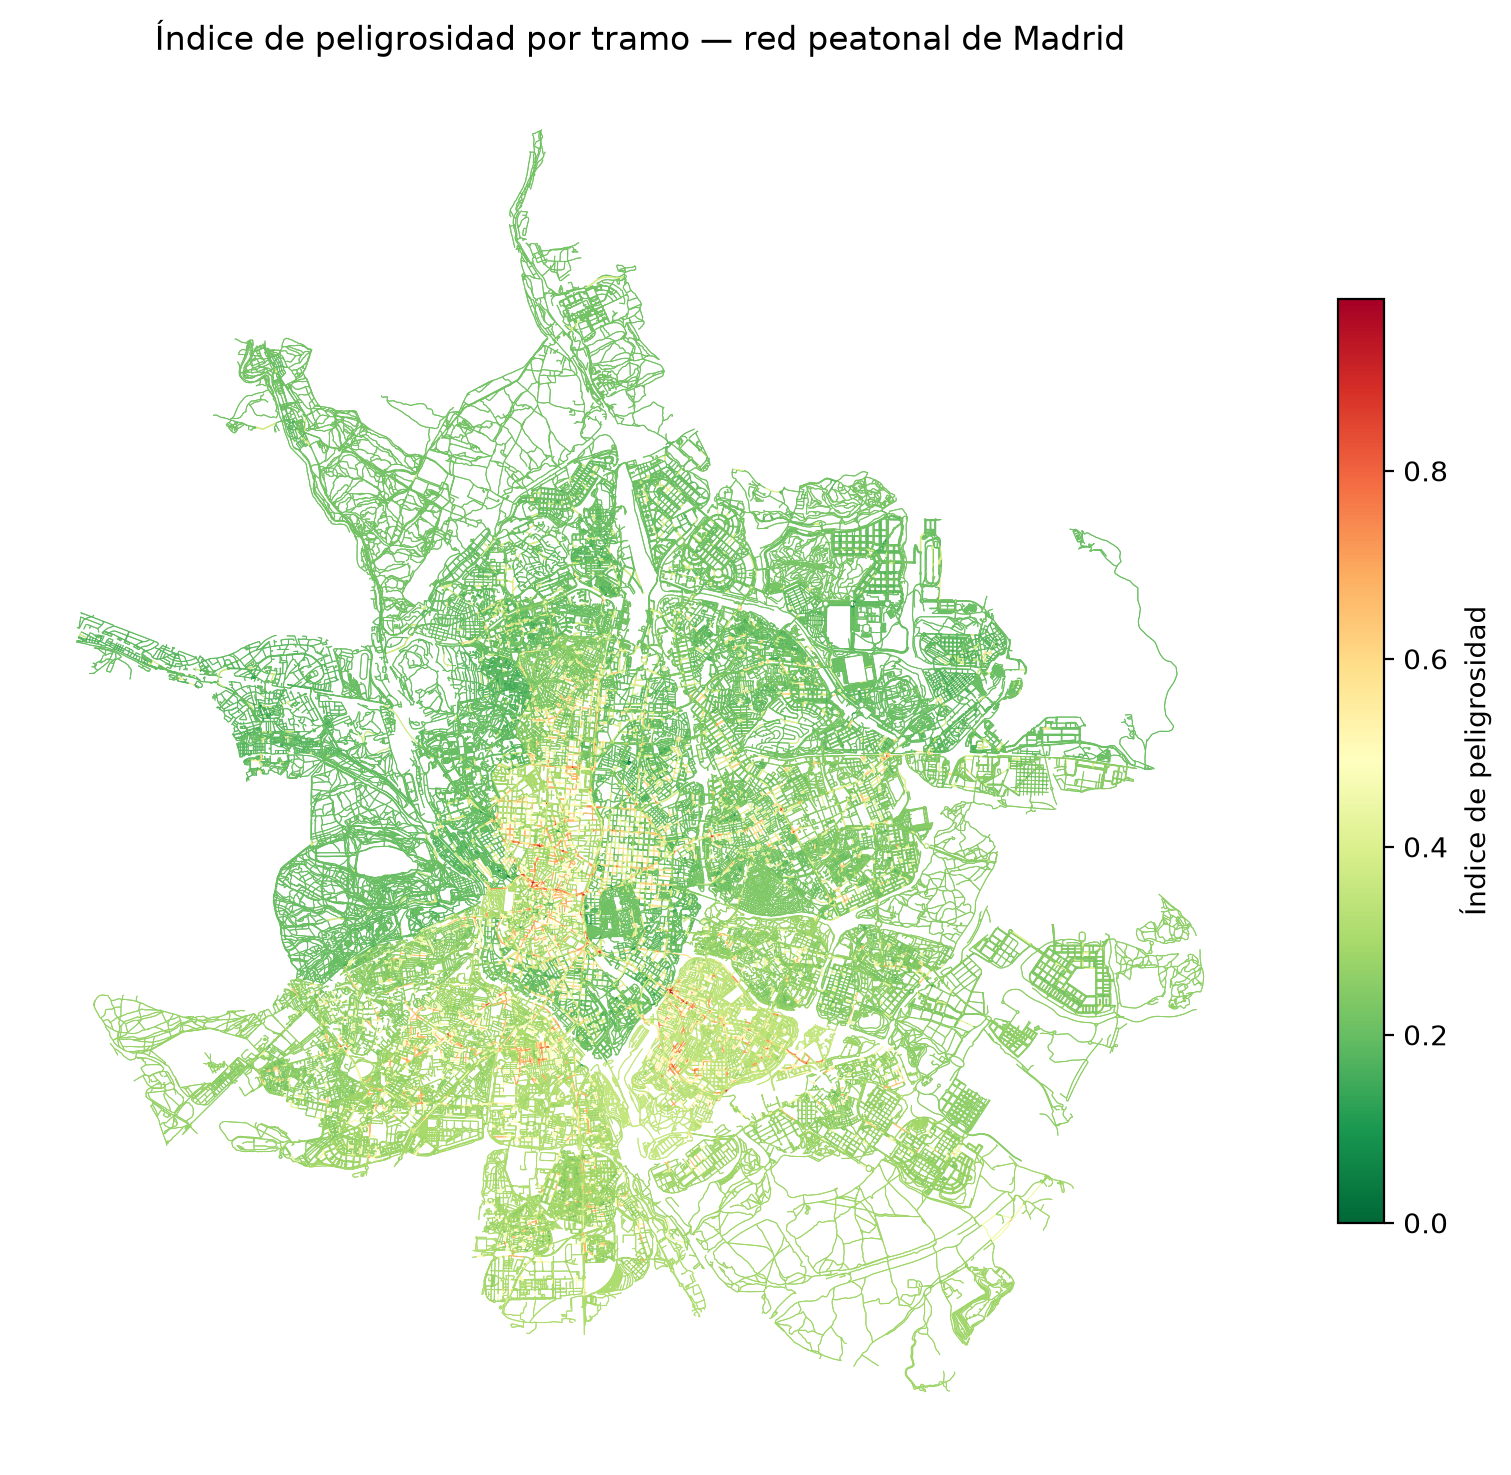
\includegraphics[width=0.8\textwidth]{imagenes/mapa_peligrosidad.png}
\caption{Índice de peligrosidad $p(e)$ por tramo en la red peatonal de Madrid (amarillo pálido: bajo, rojo oscuro: alto). Generado por \texttt{scripts/10\_mapa\_peligrosidad.py}.}
\label{fig:mapa_peligrosidad}
\end{figure}

% -----------------------------------------------------------------------
% 3.6 IMPLEMENTACIÓN DEL ENRUTAMIENTO
% -----------------------------------------------------------------------
\section{Implementación del enrutamiento seguro}
\label{sec:enrutamiento}

Una vez calculado el coste seguro para todas las aristas del grafo (Sección~\ref{subsec:coste_enrutamiento}), el enrutamiento se implementa mediante la función \texttt{pgr\_dijkstra} de pgRouting. Esta función recibe como entrada el grafo ponderado (en forma de consulta SQL sobre la tabla de aristas con sus columnas de coste), el identificador del nodo origen y el del nodo destino, y devuelve la secuencia de aristas que forman el camino de coste mínimo.

Antes de invocar \texttt{pgr\_dijkstra} es necesario resolver los dos puntos que introduce el usuario (un par de coordenadas de longitud y latitud) al nodo de la red más cercano. Esta operación se resuelve con el operador de vecino más cercano de PostGIS sobre la tabla \texttt{nodes}:

\begin{lstlisting}[style=SQL, caption={Nodo de la red más cercano a un punto dado.}, label={lst:nodo-cercano}]
SELECT osmid FROM nodes
ORDER BY geom <-> ST_SetSRID(ST_MakePoint(:lon, :lat), 4326)
LIMIT 1;
\end{lstlisting}

La consulta de enrutamiento propiamente dicha tiene la siguiente estructura:

\begin{lstlisting}[style=SQL, caption={Consulta pgRouting para el cálculo de la ruta segura, acotada a la ventana geográfica de origen y destino.}, label={lst:pgrouting}]
SELECT r.edge, e.geom, e.length, e.indice_peligrosidad
FROM pgr_dijkstra(
    -- :query construye en Python la consulta de aristas ya con
    -- la ventana geográfica (lon_min, lat_min, lon_max, lat_max
    -- y margen) resuelta a valores concretos, p. ej.:
    -- 'SELECT id, source, target, cost_seguro AS cost,
    --         reverse_cost_seguro AS reverse_cost
    --  FROM edges
    --  WHERE geom && ST_Expand(ST_MakeEnvelope(
    --      lon_min, lat_min, lon_max, lat_max, 4326), margen)'
    :query,
    :origen_id, :destino_id,
    directed => false
) r
JOIN edges e ON e.id = r.edge
ORDER BY r.seq;
\end{lstlisting}

El parámetro \texttt{directed => false} indica que el grafo se trata como no dirigido (Sección~\ref{sec:modelado_red}), por lo que \texttt{pgr\_dijkstra} puede recorrer cada arista en cualquier sentido usando indistintamente \texttt{cost} o \texttt{reverse\_cost} —en este sistema, siempre iguales—. Las filas resultantes se agregan en Python para reconstruir la geometría completa de la ruta y calcular sus estadísticas agregadas: distancia total, duración estimada (a una velocidad peatonal de referencia de 5\,km/h) y una media ponderada por longitud del índice de peligrosidad y del resto de indicadores de cada tramo recorrido.

Para el cálculo de la ruta más corta convencional (usada como referencia comparativa en el visor y en la validación), se utiliza la misma función pero sustituyendo las columnas de coste seguro por \texttt{cost} y \texttt{reverse\_cost}, que contienen directamente la longitud del tramo sin penalización alguna.

\subsection{Acotación geográfica de la consulta y elección del algoritmo}
\label{subsec:optimizacion_enrutamiento}

La primera versión de la consulta anterior no incluía la cláusula \texttt{WHERE}: se le pasaba a \texttt{pgr\_dijkstra} la red completa (\texttt{SELECT id, source, target, cost, reverse\_cost FROM edges}, sin condición alguna), delegando en el propio algoritmo la tarea de ignorar las zonas irrelevantes del grafo. Medido con \texttt{EXPLAIN ANALYZE} sobre la base de datos del proyecto (174\,394 nodos, 524\,292 aristas), esa consulta sin acotar tarda entre 1,5 y 1,9\,s por criterio, independientemente de lo corta que sea la ruta resultante, porque \texttt{pgr\_dijkstra} debe leer y materializar las 524\,292 filas de \texttt{edges} en cada invocación antes de empezar siquiera a buscar el camino.

La solución adoptada acota esa consulta a una ventana geográfica alrededor de origen y destino, apoyándose en el índice espacial \texttt{idx\_edges\_geom} (Sección~\ref{sec:modelado_red}) mediante el operador de solapamiento \texttt{\&\&}: el margen de la ventana es como mínimo de $0{,}01^\circ$ (aproximadamente 1\,km) y crece proporcionalmente a la distancia entre los dos puntos, para dar margen suficiente a los desvíos que introduce el criterio de ruta segura. Si la ventana excluyera por error el único camino posible entre dos puntos —por ejemplo, un cruce obligatorio muy alejado de la línea recta entre origen y destino—, \texttt{calcular\_ruta()} repite la consulta sin acotar antes de concluir que no existe ruta, de modo que la optimización nunca puede producir un resultado peor que antes, como mucho más lento en ese caso límite. Se comprobó, comparando la secuencia exacta de tramos devuelta con y sin acotar sobre varios pares origen-destino de distinta longitud, que ambas versiones producen la misma ruta; la acotación solo reduce el volumen de datos que \texttt{pgr\_dijkstra} tiene que leer, sin alterar el resultado. El efecto en los tiempos medidos es sustancial:

\begin{table}[h]
\centering
\begin{tabular}{lrr}
\hline
\textbf{Trayecto} & \textbf{Sin acotar} & \textbf{Acotado} \\
\hline
Corto (Puerta del Sol -- Atocha, 1,9\,km) & 1,5\,s & 0,1--0,3\,s \\
Largo (10,8\,km) & 1,9\,s & 0,7\,s \\
\hline
\end{tabular}
\caption{Tiempo de ejecución de \texttt{pgr\_dijkstra} con y sin acotar la consulta de aristas, por criterio de coste.}
\label{tab:optimizacion_dijkstra}
\end{table}

Antes de adoptar esta solución se evaluó también sustituir \texttt{pgr\_dijkstra} por \texttt{pgr\_aStar}, la variante de pgRouting que incorpora la heurística de distancia en línea recta descrita en la Sección~\ref{subsec:grafos} (dado que el coste seguro nunca es inferior a la longitud real del tramo —Sección~\ref{subsec:coste_enrutamiento}—, esa heurística es admisible también para el criterio de ruta segura, y \texttt{pgr\_aStar} garantiza por tanto encontrar la misma ruta óptima). Sin embargo, medido sobre los mismos trayectos, \texttt{pgr\_aStar} resultó sistemáticamente más lento que \texttt{pgr\_dijkstra}, tanto acotado (0,2\,s frente a 0,1\,s) como sin acotar (2,3\,s frente a 1,5\,s): \texttt{pgr\_aStar} necesita además las coordenadas de los nodos de cada arista para evaluar la heurística, lo que obliga a añadir dos \texttt{JOIN} contra la tabla \texttt{nodes} en la consulta de entrada, y ese coste adicional supera con creces el ahorro de explorar menos nodos durante la búsqueda. En otras palabras: el cuello de botella de este sistema nunca fue el algoritmo de búsqueda en sí, sino el volumen de datos que hay que leer antes de poder empezar a buscar, por lo que se mantiene \texttt{pgr\_dijkstra} y se opta por acotar la consulta de entrada en lugar de cambiar de algoritmo.

% -----------------------------------------------------------------------
% 3.7 PROTOTIPO DEL VISOR CARTOGRÁFICO
% -----------------------------------------------------------------------
\section{Prototipo del visor cartográfico}
\label{sec:visor}

El prototipo de visor cartográfico se desarrolla como una aplicación web de una sola página (\textit{Single Page Application}) utilizando \textbf{Leaflet} como biblioteca de mapas. La arquitectura del prototipo es la siguiente:

\begin{itemize}
    \item \textbf{Frontend}: página HTML con JavaScript que carga el mapa base de OpenStreetMap mediante Leaflet y ofrece tres formas de indicar el origen y el destino: un buscador de direcciones con autocompletado, un botón de geolocalización del navegador, y clic directo sobre el mapa (con geocodificación inversa para mostrar la dirección resultante). Las peticiones al backend se realizan mediante llamadas \texttt{fetch} asíncronas.
    \item \textbf{Backend}: servidor ligero en Python (Flask) con tres rutas: \texttt{GET /api/ruta}, que recibe las coordenadas de origen y destino, resuelve los nodos más cercanos, lanza las dos consultas de enrutamiento (segura y rápida) contra la base de datos y devuelve las geometrías resultantes en GeoJSON junto con sus estadísticas; y \texttt{GET /api/geocode} y \texttt{GET /api/geocode/inverso}, que actúan como \textit{proxy} de los servicios de geocodificación CartoCiudad (IGN) y Nominatim (OpenStreetMap), evitando exponer directamente esos servicios externos al cliente.
    \item \textbf{Visualización}: el visor ofrece dos modos de uso, seleccionables por el usuario. En el modo \textbf{simple} se dibuja únicamente la ruta segura, con su distancia, duración estimada y una insignia cualitativa del nivel de seguridad (obtenida discretizando el índice de peligrosidad medio de la ruta). En el modo \textbf{detallado} se dibujan ambas rutas sobre el mapa —en verde la segura, en azul discontinuo la rápida— junto con una tabla comparativa tramo a tramo de todos los indicadores descritos en la Sección~\ref{sec:funcion_coste} (siniestralidad, atropellos, iluminación y vulnerabilidad), señalando en qué medida la ruta segura mejora o empeora cada uno respecto a la ruta rápida.
\end{itemize}

A diferencia del planteamiento inicial, el prototipo implementado \textbf{no incluye un selector de franja horaria}, de forma coherente con la ausencia de esa dimensión en la función de coste (Sección~\ref{sec:vision_general}).
\chapter{Metodología e implementación}
\label{cap:metodologia}

El Capítulo~\ref{cap:propuesta} describió \textit{qué} se propone construir y con qué diseño. Este capítulo describe \textit{cómo} se ha llevado esa propuesta a la práctica: la metodología de trabajo seguida durante el desarrollo, el entorno y las herramientas técnicas empleadas, el esquema completo de la base de datos espacial resultante, y la organización del código fuente del proyecto, tanto de los procesos ETL como del prototipo de visor web.

% -----------------------------------------------------------------------
% 4.1 METODOLOGÍA DE DESARROLLO
% -----------------------------------------------------------------------
\section{Metodología de desarrollo}
\label{sec:metodologia_desarrollo}

El desarrollo se ha organizado siguiendo un enfoque \textbf{incremental por fuente de datos}: en lugar de diseñar de antemano el esquema completo de la base de datos y cargar todas las fuentes a la vez, cada fuente de riesgo se ha incorporado como un incremento independiente, verificado antes de pasar al siguiente. Esto se refleja directamente en la numeración de los scripts de \texttt{scripts/}, que documenta el orden real en que se desarrolló el sistema:

\begin{enumerate}
    \item \texttt{01\_download\_osm.py} — descarga de la red viaria peatonal con \texttt{osmnx}.
    \item \texttt{02\_load\_osm\_to\_db.py} — carga de nodos y aristas en PostgreSQL/PostGIS.
    \item \texttt{03\_load\_farolas.py} — carga de la iluminación pública y cálculo del indicador por tramo.
    \item \texttt{04\_load\_accidentes.py} — carga de accidentes y cálculo de los indicadores de siniestralidad y atropellos.
    \item \texttt{05\_load\_vulnerabilidad.py} — carga del Índice Iguala Madrid por distrito.
    \item \texttt{06\_load\_distritos.py} — carga de los polígonos de distrito y join espacial tramo-distrito.
    \item \texttt{07\_calcular\_indice\_seguridad.py} — combinación de los indicadores anteriores en el índice de peligrosidad y el coste seguro.
    \item \texttt{08\_calcular\_ruta.py} y \texttt{rutas.py} — algoritmo de enrutamiento, primero como script de línea de comandos y después como módulo reutilizable.
\end{enumerate}

Esta organización tiene una consecuencia directa sobre el esquema de la base de datos: la tabla \texttt{edges} no nace con todas sus columnas, sino que se \textbf{amplía progresivamente} a medida que cada nueva fuente de datos aporta un indicador adicional, mediante sentencias \texttt{ALTER TABLE ADD COLUMN IF NOT EXISTS} en el script SQL de cada fuente (Sección~\ref{sec:esquema_bd}).

Cada script sigue además el mismo patrón de \textbf{idempotencia}: al inicio comprueba si los datos correspondientes ya están cargados (mediante un \texttt{SELECT count(*)} sobre la tabla destino) y, si es así, no hace nada, salvo que una variable \texttt{OVERWRITE} se ponga explícitamente a \texttt{True}. Esto permite ejecutar el pipeline completo repetidamente durante el desarrollo —por ejemplo, tras corregir un error en un script posterior— sin volver a descargar o recalcular lo ya procesado, y sin arriesgarse a duplicar filas por una ejecución accidental.

Tras cada incremento se ha aplicado una \textbf{verificación de control} mediante consultas SQL directas: recuento de filas cargadas, rango de valores de los indicadores calculados, y proporción de tramos afectados (por ejemplo, comprobar que el 100\,\% de los tramos quedan asignados a un distrito tras el \textit{join} espacial, o que la distribución del índice de peligrosidad resultante cae dentro de $[0, 1]$). Esta práctica ha permitido detectar durante el desarrollo, entre otros, el problema de las densidades desproporcionadas en tramos de longitud casi nula que motivó el recorte al percentil 99 descrito en la Sección~\ref{subsec:transformacion}.

Por último, el proyecto se ha versionado con \textbf{Git} desde su inicio, con un commit por hito funcional (una fuente de datos cargada, el índice de seguridad calculado, el algoritmo de enrutamiento funcionando, cada mejora del visor web), lo que ha permitido reconstruir con precisión, ya en fase de redacción de esta memoria, el orden real en que se tomaron las decisiones de diseño.

% -----------------------------------------------------------------------
% 4.2 ENTORNO Y HERRAMIENTAS DE DESARROLLO
% -----------------------------------------------------------------------
\section{Entorno y herramientas de desarrollo}
\label{sec:entorno_herramientas}

La Tabla~\ref{tab:stack} resume las principales tecnologías y versiones empleadas en el desarrollo.

\begin{table}[h]
\centering
\begin{tabular}{ll}
\hline
\textbf{Componente} & \textbf{Versión} \\
\hline
PostgreSQL & 16 \\
PostGIS & 3.4 \\
pgRouting & 3.6 \\
Python & 3.12 \\
osmnx & 2.1.0 \\
GeoPandas & 1.1.3 \\
Pandas & 3.0.3 \\
SQLAlchemy & 2.0.43 \\
GeoAlchemy2 & 0.18.0 \\
psycopg2-binary & 2.9.10 \\
Flask & 3.1.3 \\
Leaflet & 1.9.4 \\
\hline
\end{tabular}
\caption{Principales componentes del \textit{stack} tecnológico y versión utilizada.}
\label{tab:stack}
\end{table}

El entorno de desarrollo Python se gestiona mediante un entorno virtual (\texttt{venv}) aislado del sistema, con las dependencias fijadas por versión exacta en \texttt{requirements.txt} para garantizar la reproducibilidad del entorno. Las credenciales de acceso a la base de datos (usuario, contraseña, host, puerto y nombre de la base de datos \texttt{safe\_maps}) se externalizan en un fichero \texttt{.env}, cargado en tiempo de ejecución mediante \texttt{python-dotenv} y excluido explícitamente del control de versiones, de forma que ningún secreto queda expuesto en el repositorio público del proyecto.

% -----------------------------------------------------------------------
% 4.3 ESQUEMA DE LA BASE DE DATOS
% -----------------------------------------------------------------------
\section{Esquema de la base de datos espacial}
\label{sec:esquema_bd}

La base de datos \texttt{safe\_maps} está compuesta por seis tablas, cada una introducida por el script ETL de su fuente de datos correspondiente (Sección~\ref{sec:metodologia_desarrollo}). La Tabla~\ref{tab:tablas_bd} resume su propósito y volumen tras la carga completa.

\begin{table}[h]
\centering
\small
\begin{tabular}{lp{6.5cm}r}
\hline
\textbf{Tabla} & \textbf{Contenido} & \textbf{Filas} \\
\hline
\texttt{nodes} & Nodos de la red viaria (intersecciones) & 174\,394 \\
\texttt{edges} & Tramos de calle, con los indicadores de riesgo y el coste de enrutamiento & 524\,292 \\
\texttt{farolas} & Unidades luminosas del alumbrado público & 233\,309 \\
\texttt{accidentes} & Accidentes de tráfico 2023-2025, uno por expediente & 63\,042 \\
\texttt{vulnerabilidad\_distritos} & Índice Iguala por distrito (año 2024) & 21 \\
\texttt{distritos} & Polígonos administrativos de los distritos & 21 \\
\hline
\end{tabular}
\caption{Tablas de la base de datos \texttt{safe\_maps} y su volumen tras la carga completa.}
\label{tab:tablas_bd}
\end{table}

\texttt{nodes} y \texttt{edges} constituyen el grafo viario propiamente dicho (Sección~\ref{sec:modelado_red}) y son las únicas tablas con la estructura de nodos/aristas que exige pgRouting. Las cuatro tablas restantes son fuentes de datos auxiliares que \textbf{no participan directamente en \texttt{pgr\_dijkstra}}: su función es aportar, mediante uniones espaciales o por clave de distrito, los valores con los que se rellenan las columnas de indicadores de \texttt{edges}. La Tabla~\ref{tab:columnas_edges} detalla las columnas de \texttt{edges}, agrupadas según el script que las incorpora.

\begin{table}[h]
\centering
\small
\begin{tabular}{p{4cm}p{5.2cm}p{3cm}}
\hline
\textbf{Columnas} & \textbf{Descripción} & \textbf{Origen} \\
\hline
\texttt{\small id, u, v, key, source, target, highway, name, oneway, length, cost, reverse\_cost, geom} & Identificadores del tramo y de sus nodos extremo, atributos de OSM y geometría (\texttt{cost}/\texttt{reverse\_cost} = \texttt{length}) & \texttt{\small 02\_load\_osm\_to\_db} \\
\hline
\texttt{num\_farolas, farolas\_100m} & Nº de farolas en el buffer y su densidad & \texttt{\small 03\_load\_farolas} \\
\hline
\texttt{\small num\_accidentes, accidentes\_100m, num\_atropellos} & Nº de accidentes y de atropellos en el buffer, y densidad de accidentes & \texttt{\small 04\_load\_accidentes} \\
\hline
\texttt{cod\_distrito} & Distrito asignado por \textit{join} espacial & \texttt{\small 06\_load\_distritos} \\
\hline
\texttt{\small indice\_peligrosidad, cost\_seguro, reverse\_cost\_seguro} & Índice de peligrosidad (Ecuación~\ref{eq:coste}) y coste de enrutamiento seguro & \texttt{\small 07\_calcular\_}\newline\texttt{\small indice\_seguridad} \\
\hline
\end{tabular}
\caption{Columnas de \texttt{edges}, agrupadas por el script que las incorpora.}
\label{tab:columnas_edges}
\end{table}

\begin{sloppypar}
Todas las tablas con columna de geometría (\texttt{nodes}, \texttt{edges}, \texttt{farolas}, \texttt{accidentes}, \texttt{distritos}) tienen un índice espacial \texttt{GIST} sobre dicha columna, imprescindible para que las consultas de proximidad (\texttt{ST\_DWithin}, \texttt{ST\_Within}, el operador de vecino más cercano \texttt{<->}) utilizadas en el proceso ETL y en el enrutamiento se resuelvan en tiempo razonable sobre una red de más de medio millón de tramos. \texttt{edges} tiene además índices B-tree sobre \texttt{source} y \texttt{target}, requeridos por pgRouting para resolver eficientemente los recorridos del grafo. El código SQL completo de creación de cada tabla se encuentra en \texttt{sql/01\_schema.sql} a \texttt{sql/06\_indice\_seguridad.sql}.
\end{sloppypar}

% -----------------------------------------------------------------------
% 4.4 ORGANIZACIÓN DEL CÓDIGO
% -----------------------------------------------------------------------
\section{Organización del código fuente}
\label{sec:organizacion_codigo}

El repositorio del proyecto se organiza en los siguientes directorios principales:

\begin{itemize}
    \item \texttt{scripts/} — los ocho scripts ETL y de cálculo descritos en la Sección~\ref{sec:metodologia_desarrollo}, más el módulo \texttt{rutas.py} y los scripts \texttt{09\_evaluacion.py} y \texttt{10\_mapa\_peligrosidad.py}, usados respectivamente para la evaluación comparativa del Capítulo~\ref{cap:pruebas} y para generar la Figura~\ref{fig:mapa_peligrosidad}.
    \item \texttt{sql/} — un fichero de esquema SQL por cada fuente de datos, ejecutado por su script correspondiente al inicio de cada ejecución.
    \item \texttt{data/raw/} y \texttt{data/processed/} — datos originales descargados y datos derivados (como las rutas de ejemplo exportadas a GeoJSON), excluidos del control de versiones por su tamaño.
    \item \texttt{web/} — el prototipo de visor cartográfico (Sección~\ref{sec:backend_visor}).
    \item \texttt{docs/} — la presente memoria, en \LaTeX.
\end{itemize}

\begin{sloppypar}
Todos los scripts de \texttt{scripts/} comparten una misma estructura: resuelven la ruta base del proyecto de forma independiente del directorio de trabajo actual (\texttt{Path(\_\_file\_\_).parent.parent}), cargan las credenciales desde \texttt{.env}, ejecutan el esquema SQL de su fuente de datos, y aplican el patrón de idempotencia descrito en la Sección~\ref{sec:metodologia_desarrollo}. Esta redundancia deliberada entre scripts —en lugar de extraer, por ejemplo, la creación de la conexión a una función compartida— responde a que cada script está pensado para poder leerse y ejecutarse de forma autónoma, sin necesidad de entender el resto del pipeline; el único código realmente compartido es \texttt{rutas.py}, que expone la función \texttt{calcular\_ruta()} usada tanto por el script de línea de comandos \texttt{08\_calcular\_ruta.py} como por el backend del visor web, evitando así duplicar la lógica de enrutamiento —la única parte del sistema con dos consumidores distintos.
\end{sloppypar}

% -----------------------------------------------------------------------
% 4.5 IMPLEMENTACIÓN DEL BACKEND DEL VISOR
% -----------------------------------------------------------------------
\section{Implementación del backend del visor}
\label{sec:backend_visor}

El backend del prototipo se implementa como una aplicación \textbf{Flask} de un único fichero (\texttt{web/app.py}), que expone cuatro rutas HTTP:

\begin{itemize}
    \item \texttt{GET /} — sirve la página HTML del visor.
    \item \texttt{GET /api/ruta} — recibe las coordenadas de origen y destino como parámetros de consulta e invoca \texttt{calcular\_ruta()} (Sección~\ref{sec:enrutamiento}) una vez por cada criterio (\texttt{rapida} y \texttt{segura}), en paralelo mediante un \texttt{ThreadPoolExecutor} —cada hilo con su propia conexión a la base de datos, ya que los objetos \texttt{Connection} de SQLAlchemy no son seguros para compartir entre hilos—, y devuelve ambos resultados en un único objeto JSON.
    \item \texttt{GET /api/geocode} — recibe un texto de búsqueda y consulta en paralelo (mediante un \texttt{ThreadPoolExecutor}) dos servicios de geocodificación: \textbf{CartoCiudad}, el geocodificador oficial del Instituto Geográfico Nacional basado en el Catastro, y \textbf{Nominatim}, el geocodificador de OpenStreetMap. Ambos son complementarios: CartoCiudad resuelve con precisión el número de portal de cualquier dirección de Madrid —algo que Nominatim solo consigue cuando existe en OSM un punto de interés etiquetado con ese número exacto—, mientras que Nominatim es quien indexa nombres de establecimientos y lugares (comercios, museos, monumentos) que no tienen entrada en el Catastro. Los resultados de ambos se combinan, se eliminan duplicados —tanto por proximidad de coordenadas como por coincidencia del texto mostrado— y se devuelven ya divididos en una línea principal y una línea secundaria de contexto (barrio, distrito o municipio).
    \item \texttt{GET /api/geocode/inverso} — recibe unas coordenadas y devuelve la dirección más cercana vía Nominatim, usada al hacer clic directamente sobre el mapa.
\end{itemize}

Que el backend actúe como intermediario de estos servicios, en lugar de que el cliente los consulte directamente, tiene varios motivos: permite fijar desde el servidor una cabecera \texttt{User-Agent} identificativa de la aplicación, tal como recomienda la política de uso de Nominatim; evita exponer al código JavaScript servido al navegador las URLs de los servicios externos; y es el único punto donde tiene sentido combinar y deduplicar las dos fuentes antes de enviar una única lista de sugerencias al cliente.

% -----------------------------------------------------------------------
% 4.6 IMPLEMENTACIÓN DEL FRONTEND DEL VISOR
% -----------------------------------------------------------------------
\section{Implementación del frontend del visor}
\label{sec:frontend_visor}

El frontend se implementa como una única página HTML (\texttt{web/templates/index.html}) con JavaScript nativo (sin \textit{frameworks} como React o Vue) y \textbf{Leaflet} como biblioteca de mapas, lo que mantiene el prototipo ligero y sin pasos de compilación. Sus elementos principales son:

\begin{itemize}
    \item Un \textbf{campo de búsqueda} por cada punto (origen y destino), con autocompletado contra \texttt{/api/geocode}: la petición se lanza con un \textit{debounce} de 400\,ms tras dejar de escribir, para no saturar los servicios de geocodificación con una petición por cada pulsación de tecla. Cada sugerencia se muestra en dos líneas —nombre y contexto geográfico, al estilo de los buscadores de mapas habituales— y un botón para vaciar el campo de un solo clic evita tener que borrar el texto carácter a carácter.
    \item Un botón de \textbf{geolocalización} que usa la API \texttt{navigator.geolocation} del navegador para fijar el origen en la posición actual del usuario.
    \item La posibilidad de fijar cualquiera de los dos puntos haciendo \textbf{clic directamente sobre el mapa}, con geocodificación inversa automática para mostrar la dirección resultante en el campo correspondiente.
    \item Un botón para \textbf{intercambiar} origen y destino.
    \item Dos \textbf{modos de visualización}, descritos ya en la Sección~\ref{sec:visor}: \textit{simple}, con una única ruta recomendada y una insignia cualitativa de seguridad; y \textit{detallado}, con ambas rutas superpuestas y una tabla comparativa de los indicadores de la Sección~\ref{sec:funcion_coste}.
    \item Una interfaz \textbf{adaptable (\textit{responsive})} a dispositivos móviles: por debajo de 720\,px de ancho el panel de búsqueda pasa de disposición lateral a apilada bajo el mapa, con unidades de \textit{viewport} dinámicas (\texttt{dvh}) para evitar el recorte que provoca la barra de direcciones de los navegadores móviles, y un caso específico para orientación horizontal en pantallas de poca altura.
\end{itemize}

El estado de la interfaz (puntos seleccionados, modo activo, última respuesta del servidor) se mantiene en un único objeto JavaScript en memoria, y el cambio entre modos \textit{simple} y \textit{detallado} se resuelve completamente en el cliente reutilizando la última respuesta de \texttt{/api/ruta}, sin necesidad de repetir la consulta de enrutamiento al backend.

La Figura~\ref{fig:visor_buscador} muestra el buscador de direcciones en funcionamiento: mientras el usuario escribe, el campo consulta \texttt{/api/geocode} con el \textit{debounce} descrito más arriba y despliega una lista de sugerencias acotadas al municipio de Madrid, de la que se selecciona una para fijar el origen o el destino. El ejemplo de la figura, una dirección con número de portal, ilustra precisamente el motivo de combinar ambos geocodificadores: es CartoCiudad, y no Nominatim, quien resuelve el número exacto (22) en las sugerencias mostradas.

\begin{figure}[h]
\centering
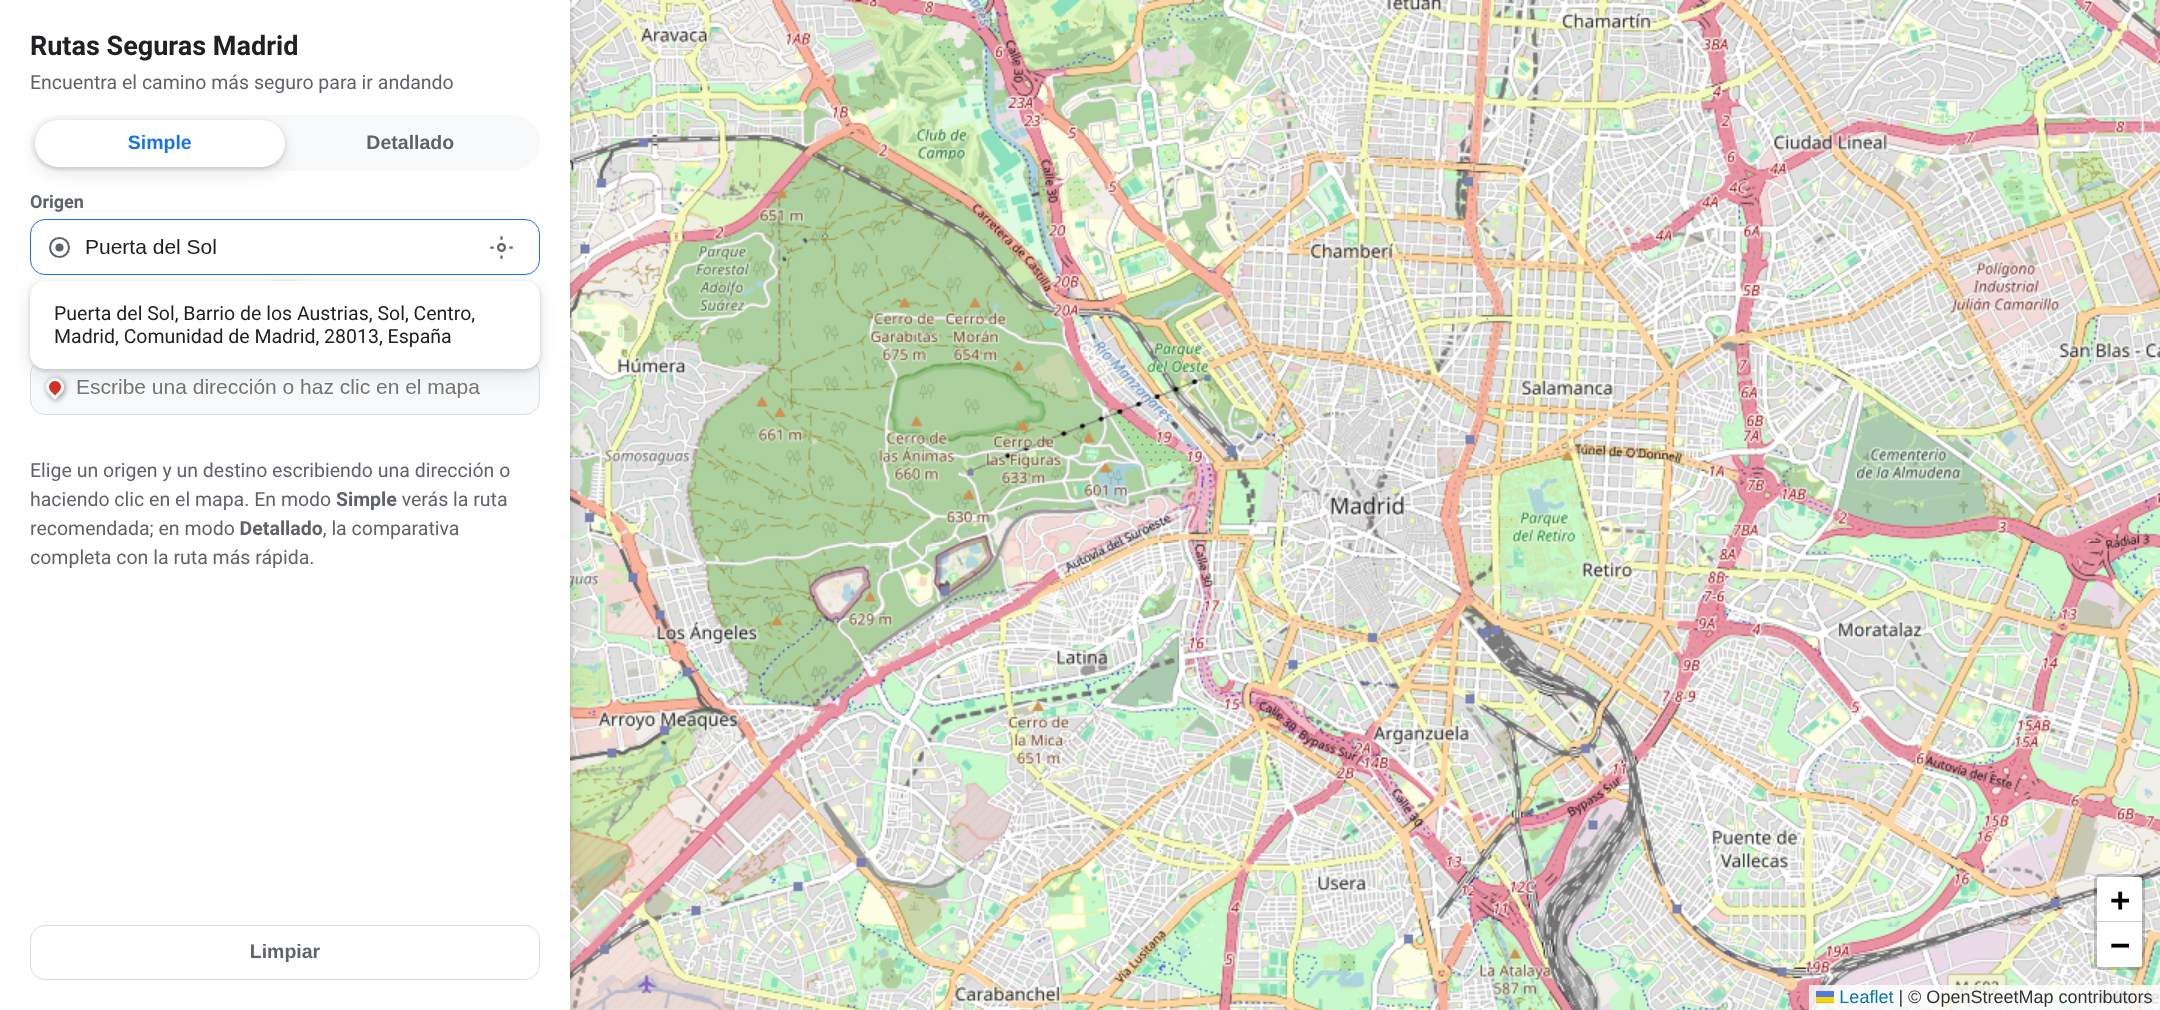
\includegraphics[width=\textwidth]{imagenes/visor_buscador.png}
\caption{Buscador de direcciones con autocompletado contra \texttt{/api/geocode}, mostrando las sugerencias para "Paseo de la Castellana 22".}
\label{fig:visor_buscador}
\end{figure}

Las Figuras~\ref{fig:visor_simple} y~\ref{fig:visor_detallado} muestran el prototipo en funcionamiento sobre el par Puerta del Sol -- Atocha, uno de los pares origen-destino que se retoman con más detalle en la evaluación del Capítulo~\ref{cap:pruebas}. En el modo simple (Figura~\ref{fig:visor_simple}) se aprecia la ruta recomendada, su distancia y duración, y la insignia cualitativa de seguridad (\textit{Segura} en este caso). En el modo detallado (Figura~\ref{fig:visor_detallado}) se superponen ambas rutas —discontinua en azul la rápida, continua en verde la segura— junto con la tabla comparativa de indicadores, cuyos valores coinciden con los recogidos más adelante en la Tabla~\ref{tab:resultados_rutas}.

\begin{figure}[h]
\centering
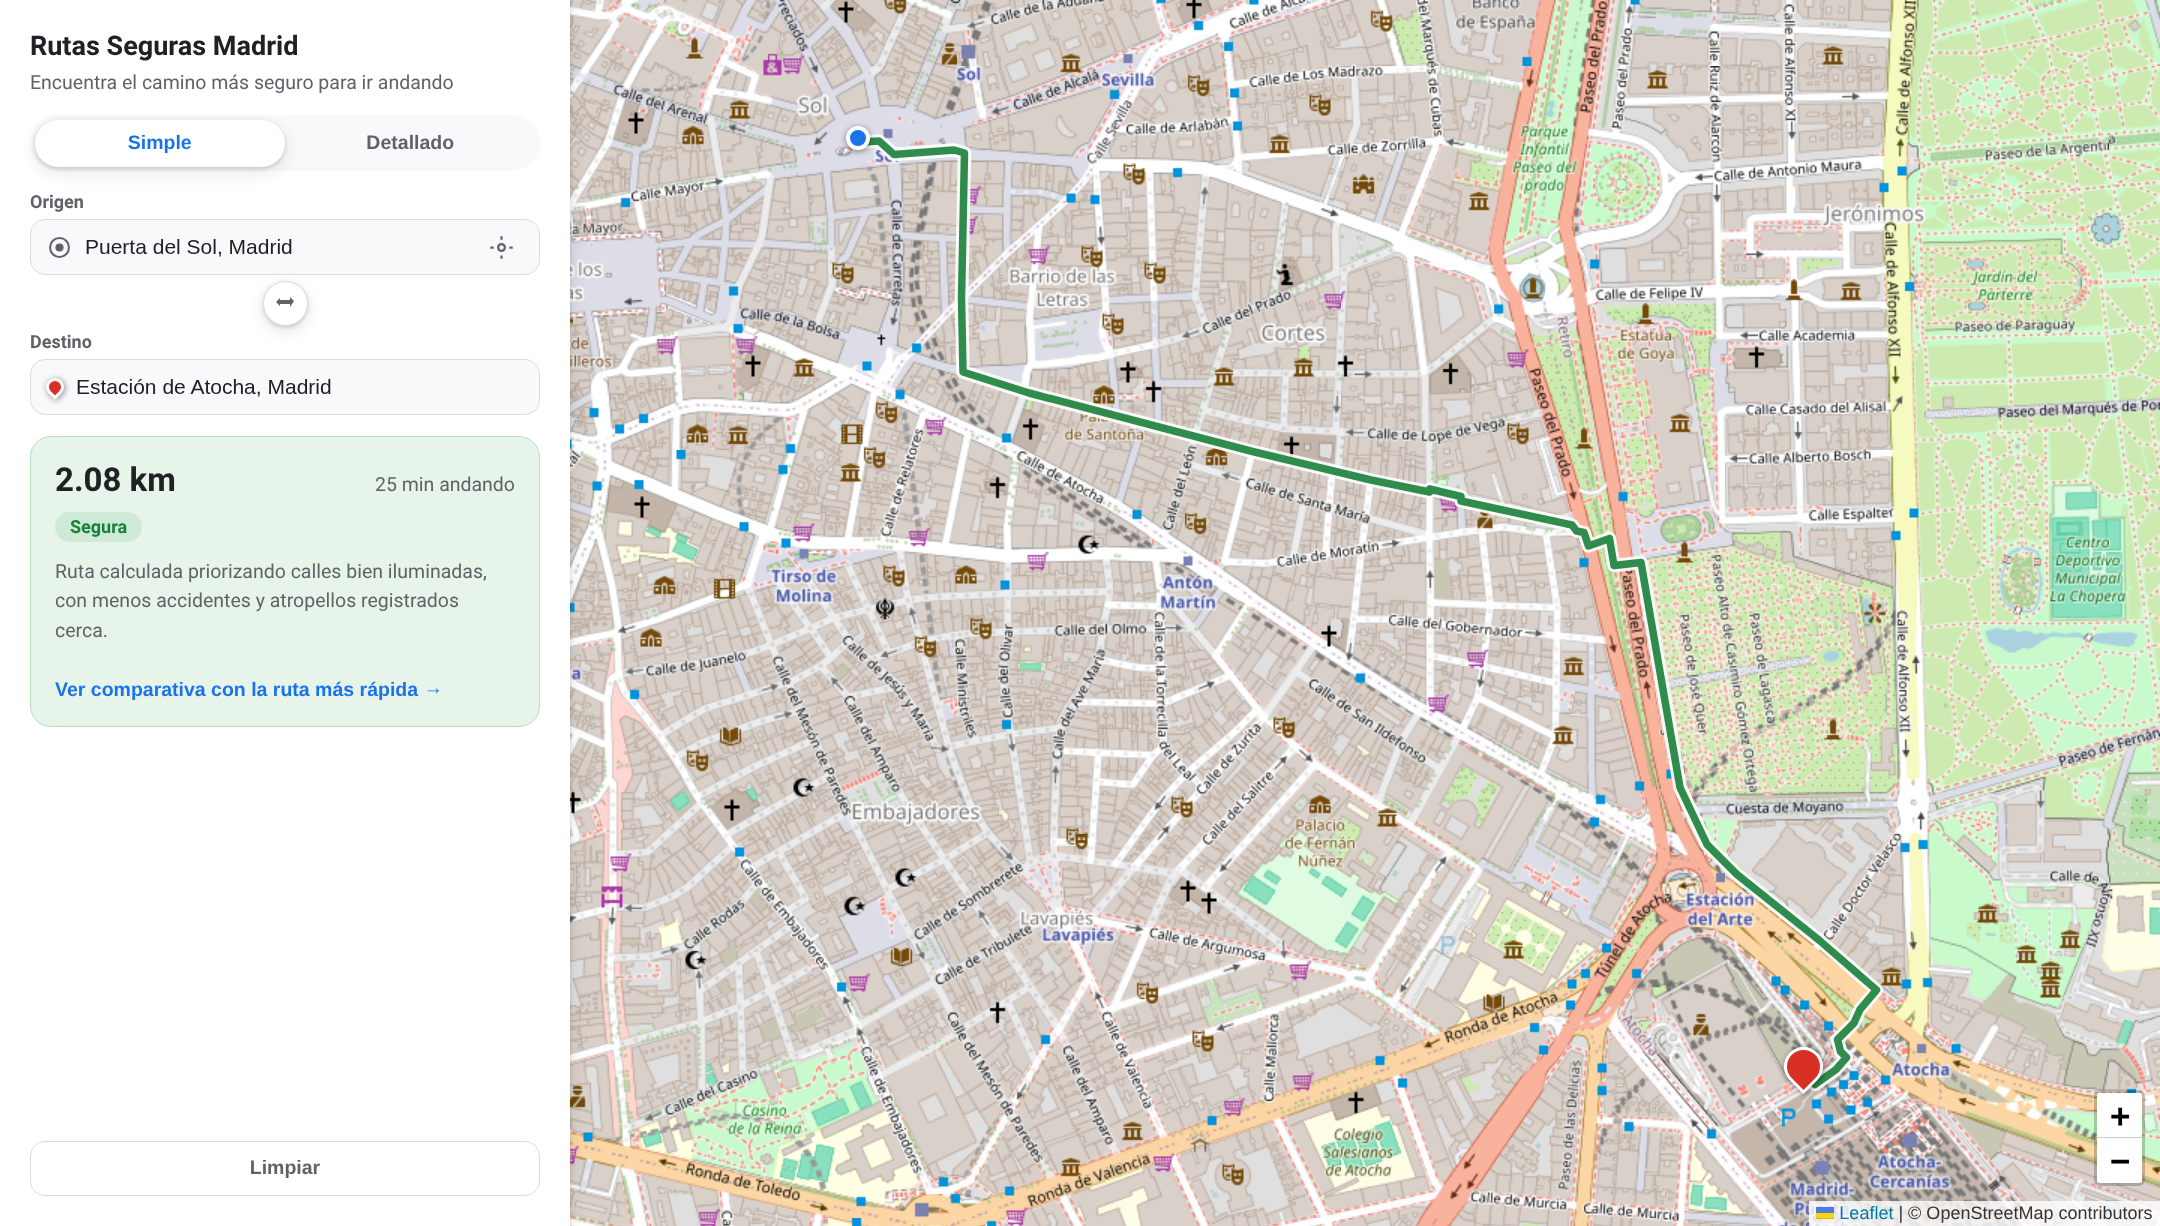
\includegraphics[width=\textwidth]{imagenes/visor_simple.png}
\caption{Visor web, modo simple, para el trayecto Puerta del Sol -- Atocha.}
\label{fig:visor_simple}
\end{figure}

\begin{figure}[h]
\centering
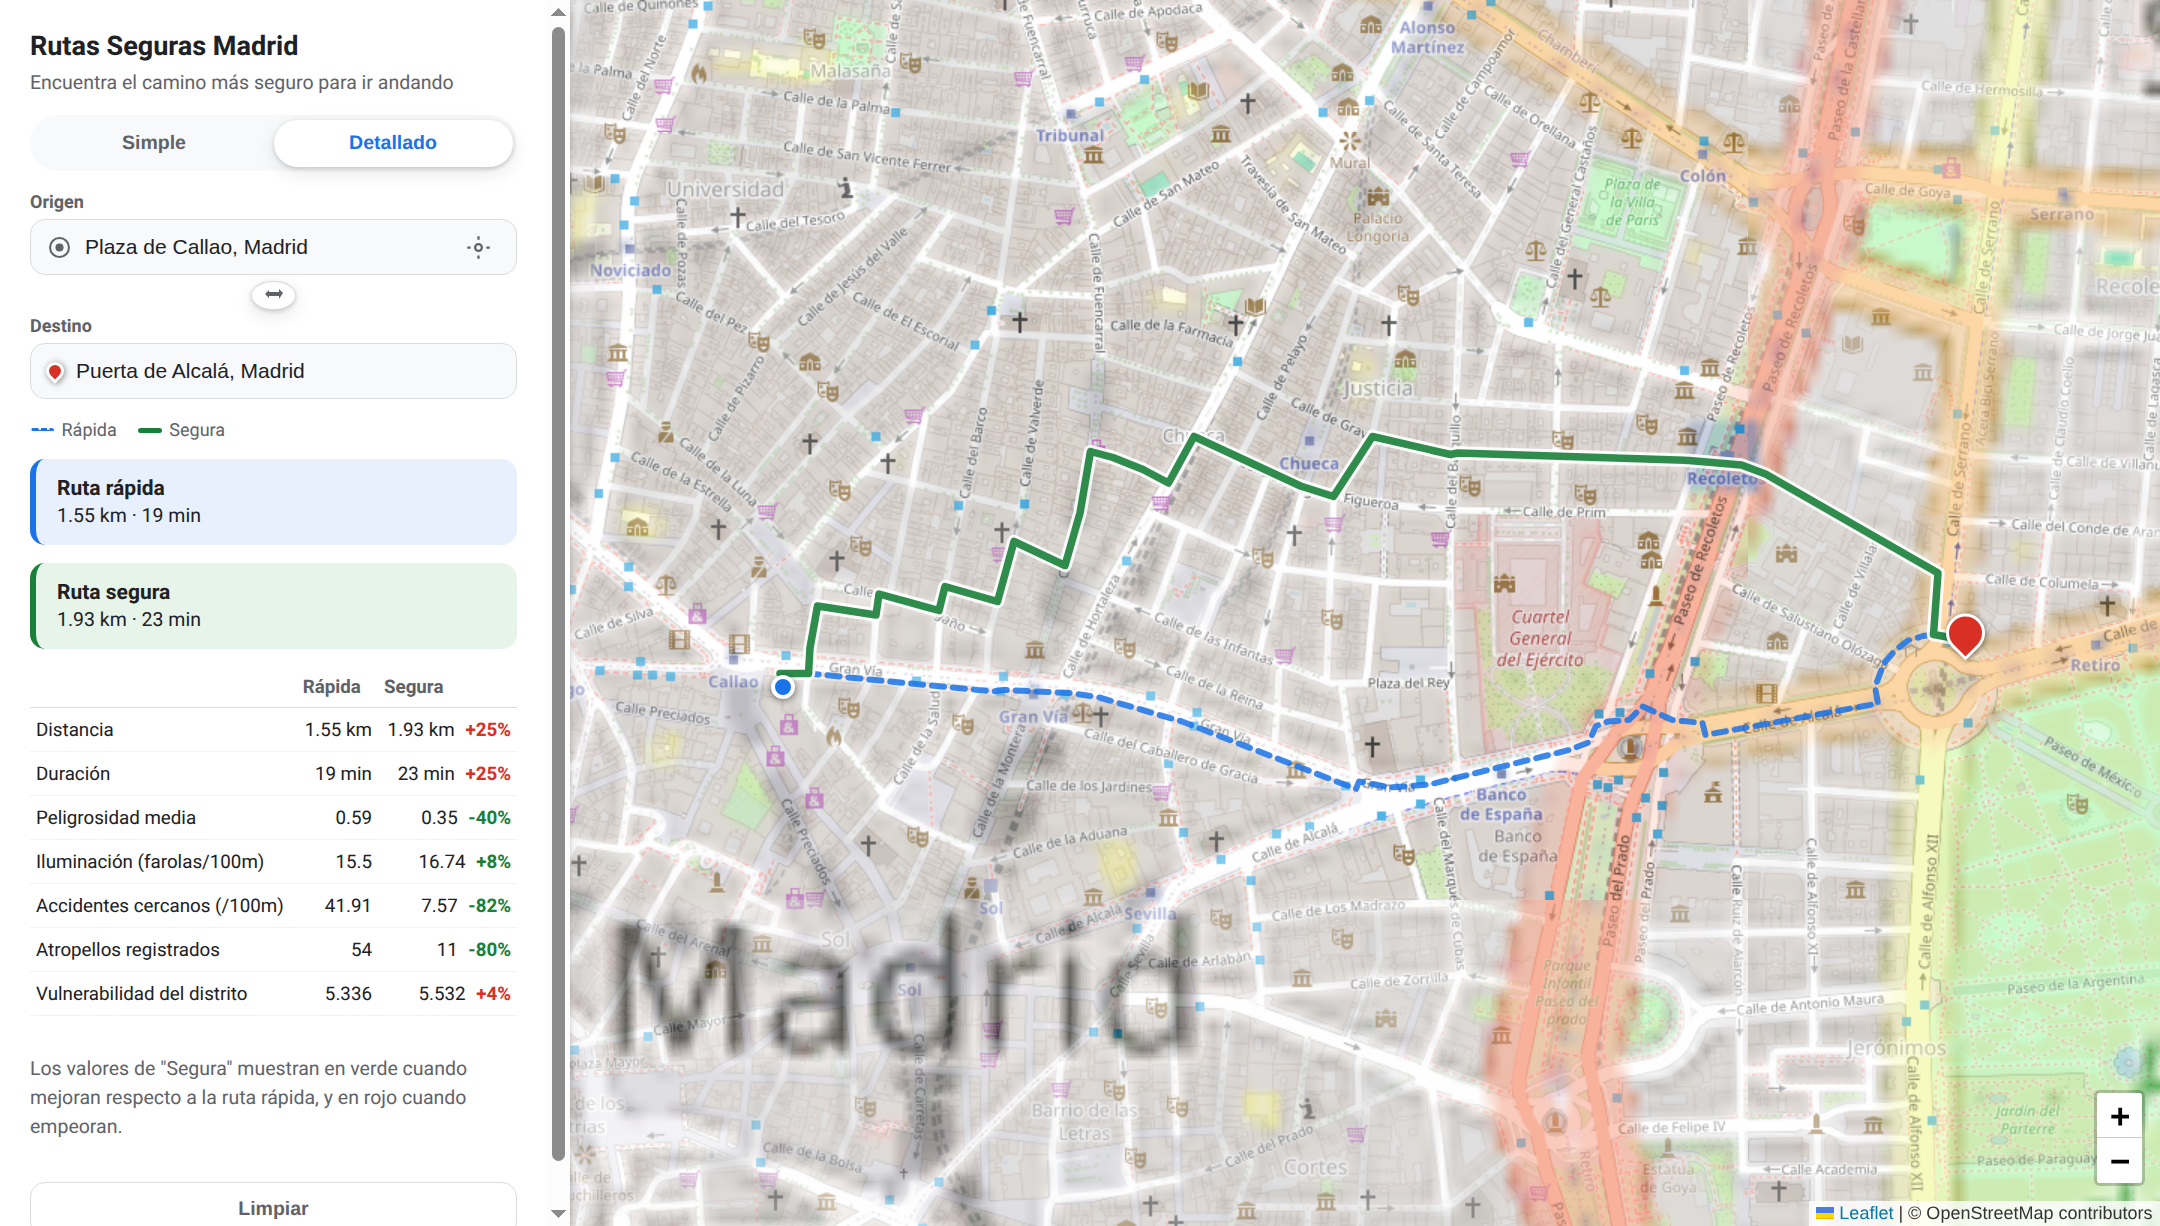
\includegraphics[width=\textwidth]{imagenes/visor_detallado.png}
\caption{Visor web, modo detallado, para el mismo trayecto: comparativa entre la ruta rápida y la ruta segura.}
\label{fig:visor_detallado}
\end{figure}

\chapter{Gestión del proyecto}
\label{cap:gestion}

Este capítulo recoge los aspectos de gestión del Trabajo Fin de Grado: la metodología de trabajo seguida para organizar el desarrollo en el tiempo disponible, la planificación temporal real del proyecto y una estimación del presupuesto asociado.

% -----------------------------------------------------------------------
% 5.1 METODOLOGÍA DE GESTIÓN
% -----------------------------------------------------------------------
\section{Metodología de gestión}
\label{sec:metodologia_gestion}

El proyecto ha sido desarrollado en su totalidad por la autora de forma individual, compaginando el trabajo con unas prácticas curriculares en empresa entre marzo y junio, y con una incorporación laboral posterior. Esta circunstancia ha condicionado directamente la forma de gestionar el proyecto: en lugar de sesiones largas de trabajo, la dedicación real ha consistido en sesiones cortas, de en torno a dos horas, dispersas de lunes a viernes a lo largo de aproximadamente seis meses (Sección~\ref{sec:planificacion_temporal}).

Dado este contexto, se descartó desde el principio recurrir a herramientas de gestión de proyectos externas (tipo Jira o Trello): su valor está en coordinar a varias personas, y en un desarrollo unipersonal como este habrían supuesto una carga de gestión (overhead) sin beneficio real. En su lugar, se siguió una planificación iterativa e incremental inspirada en metodologías ágiles y, más concretamente, en la lógica del desarrollo guiado por características (\textit{Feature-Driven Development}): cada incremento de la planificación (Sección~\ref{sec:planificacion_temporal}) se hizo coincidir con una funcionalidad completa, autocontenida y verificada antes de pasar a la siguiente, siguiendo la misma organización por fuente de datos descrita en la Sección~\ref{sec:metodologia_desarrollo} (la descarga de la red viaria, su carga en PostGIS, la incorporación sucesiva de iluminación, accidentalidad y vulnerabilidad territorial, el motor de enrutamiento con pgRouting y, por último, el visor web). Este enfoque modular, más que la disciplina de una metodología formal, respondía a una necesidad práctica: minimizar el contexto que había que recuperar mentalmente al retomar el proyecto tras varios días sin tocarlo.

En consonancia con esa misma lógica incremental, el criterio seguido para los commits de Git ha sido uno por hito funcional verificado, tal y como ya se señaló en la Sección~\ref{sec:metodologia_desarrollo}. Durante las semanas de mayor carga por las prácticas en empresa, varios hitos completados y probados localmente se acumulaban sin subir al repositorio remoto, y se integraban juntos en cuanto había un hueco para revisarlos con calma; esto explica que el historial de commits muestre concentraciones puntuales de actividad que no reflejan fielmente el reparto real del esfuerzo, más homogéneo y disperso en el tiempo de lo que el propio historial de Git sugiere. Se trata, por tanto, de una estrategia deliberada de integración de código ya estable, y no de una falta de continuidad en el desarrollo.

% -----------------------------------------------------------------------
% 5.2 PLANIFICACIÓN TEMPORAL
% -----------------------------------------------------------------------
\section{Planificación temporal}
\label{sec:planificacion_temporal}

El TFG tiene asignados 12 créditos ECTS, equivalentes de forma nominal a unas 300 horas de dedicación. La estimación de horas efectivamente invertidas, calculada a partir del ritmo real de trabajo (dos horas aproximadas, de lunes a viernes, entre principios de marzo y el 1 de septiembre), se sitúa en torno a las \textbf{270 horas}, una cifra coherente con la carga nominal de la asignatura una vez descontadas las semanas de menor dedicación por solapamiento con las prácticas en empresa.

El desarrollo se ha organizado en las siguientes ocho fases:

\begin{enumerate}
    \item \textbf{F1 - Estudio del estado del arte y definición de objetivos} (2 marzo -- 17 abril): revisión bibliográfica sobre enrutamiento seguro (Capítulo~\ref{cap:introduccion}), y definición del objetivo general, los objetivos específicos y la hipótesis de partida.
    \item \textbf{F2 - Diseño de la propuesta y selección tecnológica} (20 abril -- 1 mayo): definición de la arquitectura del sistema y elección del stack (PostgreSQL/PostGIS/pgRouting, Python, Leaflet), descrita en el Capítulo~\ref{cap:propuesta}.
    \item \textbf{F3 - Configuración del entorno y carga de la red viaria} (4 -- 29 mayo): puesta en marcha de la base de datos \texttt{safe\_maps} y desarrollo de \texttt{01\_download\_osm.py} y \texttt{02\_load\_osm\_to\_db.py}.
    \item \textbf{F4 - ETL de las fuentes de seguridad} (1 junio -- 10 julio): desarrollo de los scripts \texttt{03} a \texttt{06} (farolas, accidentes, vulnerabilidad territorial y distritos), la fase de mayor duración del proyecto por incluir cuatro fuentes de datos heterogéneas.
    \item \textbf{F5 - Índice de seguridad y motor de enrutamiento} (13 -- 31 julio): diseño de la función de coste (Sección~\ref{sec:funcion_coste}) y desarrollo de \texttt{07\_calcular\_indice\_seguridad.py}, \texttt{rutas.py} y \texttt{08\_calcular\_ruta.py}.
    \item \textbf{F6 - Prototipo del visor web} (3 -- 21 agosto): desarrollo del backend Flask y el frontend Leaflet (Secciones~\ref{sec:backend_visor} y~\ref{sec:frontend_visor}), incluyendo el rediseño posterior del buscador de direcciones (CartoCiudad y Nominatim combinados) y los modos simple/detallado.
    \item \textbf{F7 - Redacción de la memoria: capítulos 1 a 4} (20 -- 24 agosto): redacción de la introducción, el estado del arte, la propuesta y la metodología, en paralelo con el cierre de F6.
    \item \textbf{F8 - Pruebas, gestión, conclusiones y revisión final} (25 agosto -- 1 septiembre): redacción de los capítulos de pruebas y validación, gestión del proyecto y conclusiones, elaboración de apéndices y revisión final antes de la solicitud de evaluación.
\end{enumerate}

La Figura~\ref{fig:gantt} representa esta planificación mediante un diagrama de Gantt.

\begin{figure}[htbp]
\centering
\begin{ganttchart}[
    hgrid,
    vgrid,
    x unit=0.34cm,
    y unit title=0.6cm,
    y unit chart=0.6cm,
    title height=1,
    bar height=0.55,
    bar/.append style={fill=gray!60},
    bar label font=\small,
    title label font=\small\bfseries,
    milestone/.append style={fill=black}
]{1}{27}
\gantttitle{Mar}{4}
\gantttitle{Abr}{5}
\gantttitle{May}{4}
\gantttitle{Jun}{5}
\gantttitle{Jul}{4}
\gantttitle{Ago}{4}
\gantttitle{Sep}{1} \\
\ganttbar{F1 -- Estado del arte y objetivos}{1}{7} \\
\ganttbar{F2 -- Diseño y selección tecnológica}{8}{9} \\
\ganttbar{F3 -- Entorno y carga red viaria}{10}{13} \\
\ganttbar{F4 -- ETL fuentes de seguridad}{14}{19} \\
\ganttbar{F5 -- Índice y enrutamiento}{20}{22} \\
\ganttbar{F6 -- Prototipo del visor web}{23}{25} \\
\ganttbar{F7 -- Memoria (cap. 1--4)}{25}{26} \\
\ganttbar{F8 -- Pruebas, gestión y cierre}{26}{27} \\
\ganttmilestone{Solicitud de evaluación}{27}
\end{ganttchart}
\caption{Planificación temporal del proyecto por semanas (marzo -- septiembre de 2026).}
\label{fig:gantt}
\end{figure}

% -----------------------------------------------------------------------
% 5.3 ESTIMACIÓN DE RECURSOS Y PRESUPUESTO
% -----------------------------------------------------------------------
\section{Estimación de recursos y presupuesto}
\label{sec:presupuesto}

Al tratarse de un Trabajo Fin de Grado, el proyecto no ha generado ningún desembolso económico real. No obstante, se incluye a continuación una estimación orientativa de su coste si se hubiera desarrollado en un contexto profesional.

\textbf{Recursos humanos.} Se estima el coste del trabajo desarrollado tomando como referencia una tarifa de mercado para un perfil de desarrollador/analista de datos junior, aplicada a las 270 horas de dedicación estimadas en la Sección~\ref{sec:planificacion_temporal}.

\textbf{Recursos materiales.} Se contabiliza la amortización del equipo portátil personal empleado para el desarrollo, calculada de forma lineal sobre una vida útil de 4 años y prorrateada a los 6 meses de duración del proyecto.

\textbf{Software.} Todas las herramientas empleadas (PostgreSQL, PostGIS, pgRouting, Python y sus bibliotecas, Flask y Leaflet; Tabla~\ref{tab:stack}) son de código abierto y sin coste de licencia. Las fuentes de datos utilizadas (OpenStreetMap, Datos Abiertos del Ayuntamiento de Madrid, Geoportal de Madrid, Nominatim, CartoCiudad del Instituto Geográfico Nacional) son igualmente de acceso público y gratuito.

\begin{table}[htbp]
\centering
\begin{tabular}{lrrr}
\hline
\textbf{Partida} & \textbf{Cantidad} & \textbf{Coste unitario} & \textbf{Coste total} \\
\hline
Recursos humanos & 270 h & 20\,\euro/h & 5\,400\,\euro \\
Recursos materiales (amortización portátil) & 6 meses & 25\,\euro/mes & 150\,\euro \\
Software y licencias & --- & 0\,\euro & 0\,\euro \\
\hline
\textbf{Total estimado} & & & \textbf{5\,550\,\euro} \\
\hline
\end{tabular}
\caption{Estimación del presupuesto del proyecto.}
\label{tab:presupuesto}
\end{table}

No se han incluido en esta estimación los costes de electricidad o conexión a internet, por resultar difícilmente atribuibles al proyecto de forma individual, ni las horas de dirección académica del tutor, al no constituir un coste asumido por la autora.

\chapter{Pruebas y validación}
\label{cap:pruebas}

Este capítulo aborda el objetivo específico OE6 (Sección~\ref{subsec:objetivos_especificos}): evaluar cuantitativamente en qué medida la ruta segura difiere de la ruta más corta, tanto en coste de desplazamiento (distancia, tiempo) como en exposición al riesgo (índice de peligrosidad y sus componentes), y contrastar el resultado con la hipótesis de partida (Sección~\ref{subsec:hipotesis}).

% -----------------------------------------------------------------------
% 6.1 METODOLOGÍA DE EVALUACIÓN
% -----------------------------------------------------------------------
\section{Metodología de evaluación}
\label{sec:metodologia_evaluacion}

La evaluación se ha realizado calculando, para un conjunto de pares origen-destino, la ruta \textit{rápida} (criterio \texttt{cost}, Sección~\ref{sec:enrutamiento}) y la ruta \textit{segura} (criterio \texttt{cost\_seguro}) mediante la misma función \texttt{calcular\_ruta()} que expone el visor web, y comparando sus estadísticas agregadas: distancia, duración estimada, índice de peligrosidad medio, densidad media de iluminación y de accidentalidad, número total de atropellos y vulnerabilidad territorial media, todos ellos ponderados por la longitud de cada tramo recorrido (Sección~\ref{sec:enrutamiento}).

Se han seleccionado \textbf{ocho pares origen-destino} (Tabla~\ref{tab:resultados_rutas}) con dos criterios de variación deliberada: la \textbf{distancia}, desde trayectos cortos de menos de 2\,km (por ejemplo, Puerta del Sol -- Atocha) hasta trayectos largos de más de 5\,km (Plaza Elíptica -- Puente de Vallecas); y el \textbf{perfil de vulnerabilidad territorial} de los distritos atravesados, desde pares que discurren íntegramente por distritos de baja vulnerabilidad según el Índice Iguala (Moncloa, Chamartín) hasta pares que atraviesan distritos de vulnerabilidad alta (Usera, Villaverde, Puente de Vallecas; véanse los valores de \texttt{ivt\_agregado} en la Sección~\ref{sec:esquema_bd}). No se ha pretendido un muestreo aleatorio y representativo de todo el callejero de Madrid —lo que exigiría un número de pares muy superior—, sino cubrir de forma deliberada esta variabilidad para poder observar cómo cambia el comportamiento del sistema según el contexto.

El proceso está automatizado en \texttt{scripts/09\_evaluacion.py}, que sigue la misma convención de rutas y estructura que el resto de scripts del proyecto (Sección~\ref{sec:metodologia_desarrollo}): calcula ambas rutas para cada par, imprime un resumen por consola y vuelca el resultado completo en \texttt{data/processed/evaluacion\_rutas.csv} para su análisis. Todos los resultados presentados en este capítulo son directamente reproducibles ejecutando dicho script sobre la base de datos \texttt{safe\_maps}.

% -----------------------------------------------------------------------
% 6.2 RESULTADOS COMPARATIVOS
% -----------------------------------------------------------------------
\section{Resultados comparativos}
\label{sec:resultados_comparativos}

La Tabla~\ref{tab:resultados_rutas} resume, para cada par origen-destino, la distancia y el índice de peligrosidad medio de ambas rutas, junto con la variación relativa ($\Delta$) de la ruta segura respecto a la rápida, y el número total de atropellos acumulados a lo largo de cada ruta.

\begin{table}[h]
\centering
\small
\begin{tabular}{lrrrrrrr}
\hline
\textbf{Par origen-destino} & \multicolumn{3}{c}{\textbf{Distancia (m)}} & \multicolumn{3}{c}{\textbf{Peligrosidad media}} & \textbf{Atropellos} \\
 & Ráp. & Seg. & $\Delta$\,\% & Ráp. & Seg. & $\Delta$\,\% & Ráp.$\to$Seg. \\
\hline
Sol -- Atocha                    & 1\,922 & 2\,084 & +8.5  & 0.4305 & 0.3100 & -28.0 & 39 $\to$ 12 \\
Callao -- Pta.\ Alcalá           & 1\,549 & 1\,930 & +24.6 & 0.5862 & 0.3510 & -40.1 & 54 $\to$ 11 \\
N.\ Ministerios -- 4 Caminos     & 1\,557 & 1\,666 & +7.0  & 0.4726 & 0.3987 & -15.6 & 30 $\to$ 28 \\
Pza.\ Elíptica -- Pte.\ Vallecas & 5\,624 & 5\,858 & +4.2  & 0.3849 & 0.3221 & -16.3 & 63 $\to$ 30 \\
Moncloa -- C.\ Universitaria     & 1\,672 & 1\,673 & +0.0  & 0.2253 & 0.2250 & -0.1  & 14 $\to$ 14 \\
Villaverde Alto -- Usera         & 5\,101 & 5\,155 & +1.1  & 0.3529 & 0.3276 & -7.2  & 15 $\to$ 9 \\
Chamartín -- Hortaleza           & 4\,780 & 4\,818 & +0.8  & 0.2422 & 0.2342 & -3.3  & 8 $\to$ 3 \\
Vicálvaro -- V.\ Vallecas        & 4\,416 & 4\,421 & +0.1  & 0.2720 & 0.2712 & -0.3  & 6 $\to$ 6 \\
\hline
\textbf{Media de los 8 pares}    &        &        & \textbf{+5.8} &        &        & \textbf{-13.9} & \textbf{229 $\to$ 113} \\
\hline
\end{tabular}
\caption{Comparativa entre la ruta rápida y la ruta segura para los ocho pares origen-destino evaluados. La fila final agrega las variaciones porcentuales medias y la suma total de atropellos.}
\label{tab:resultados_rutas}
\end{table}

Dos lecturas agregadas de la Tabla~\ref{tab:resultados_rutas} resultan especialmente relevantes. Considerando la \textbf{distancia total} recorrida en los ocho trayectos (suma de las ocho rutas, no la media de los porcentajes individuales), la ruta segura supone un incremento del \textbf{3.7\,\%} sobre la ruta rápida (de 26\,621\,m a 27\,604\,m) —una cifra menor que la media simple de los ocho porcentajes (+5.8\,\%) porque los pares más largos, que pesan más en el total, son también los que menos se desvían en términos relativos. Considerando el número \textbf{total} de atropellos acumulados en los ocho trayectos, la ruta segura los reduce de 229 a 113, un \textbf{50.7\,\%} menos.

Se observan además dos patrones claros en función del contexto:

\begin{itemize}
    \item En los pares que discurren por \textbf{zonas céntricas de tráfico denso} (Sol -- Atocha, Callao -- Puerta de Alcalá), la ruta segura evita tramos con una accidentalidad muy superior a la media —el indicador \texttt{accidentes\_100m} pasa, en el caso Callao -- Puerta de Alcalá, de 41.9 a 7.6— a cambio de un desvío perceptible (hasta +24.6\,\% de distancia en ese mismo par). Es precisamente en estos casos donde la reducción de peligrosidad es mayor (-28.0\,\% y -40.1\,\% respectivamente).
    \item En los pares \textbf{Moncloa -- Ciudad Universitaria} y \textbf{Vicálvaro -- Villa de Vallecas}, ambas rutas son prácticamente idénticas ($\Delta$ distancia inferior al 0.1\,\%). En estas zonas, de menor densidad de red peatonal alternativa o de riesgo ya relativamente homogéneo entre las vías disponibles, el algoritmo no encuentra ningún desvío que reduzca el coste de seguridad sin penalizar en exceso la distancia, por lo que la ruta óptima según ambos criterios coincide.
\end{itemize}

% -----------------------------------------------------------------------
% 6.3 DISCUSIÓN
% -----------------------------------------------------------------------
\section{Discusión}
\label{sec:discusion_resultados}

La hipótesis de partida (Sección~\ref{subsec:hipotesis}) planteaba que es posible reducir la exposición a factores de riesgo urbano \textit{con un incremento de distancia o tiempo de recorrido asumible}. Los resultados obtenidos son consistentes con esta hipótesis: un incremento agregado del 3.7\,\% en distancia (equivalente en tiempo, al usarse una velocidad peatonal constante, Sección~\ref{sec:enrutamiento}) se corresponde con una reducción del 50.7\,\% en el número total de atropellos acumulados y de un 13.9\,\% de media en el índice de peligrosidad. Esta relación es incluso más favorable que la reportada por Sohrabi et al. \cite{sohrabi2022} para vehículos —un incremento del 8\,\% en tiempo de viaje asociado a una reducción del 23\,\% en probabilidad de accidente—, si bien ambas cifras no son directamente comparables: la de Sohrabi et al.\ mide una reducción real de probabilidad de accidente sobre datos de siniestralidad vehicular, mientras que la obtenida aquí es una reducción de un índice compuesto y ponderado (Sección~\ref{sec:funcion_coste}), calculado sobre ocho trayectos concretos y no sobre una muestra estadísticamente representativa de toda la red.

Que el desvío se mantenga moderado incluso en los pares con mayor reducción de peligrosidad (máximo +24.6\,\% de distancia) es una consecuencia directa del diseño de la función de coste: la constante $\alpha = 4$ (Ecuación~\ref{eq:coste_seguro}) limita el coste de cualquier tramo a, como máximo, cinco veces su longitud real, por lo que \texttt{pgr\_dijkstra} nunca encuentra rentable un rodeo arbitrariamente largo para evitar un único tramo peligroso; el propio valor de $\alpha$ se ajustó de forma empírica observando este comportamiento sobre varios pares origen-destino (Sección~\ref{subsec:coste_enrutamiento}), y los resultados de este capítulo confirman a posteriori, sobre un conjunto más amplio de pares, que esa elección produce desvíos perceptibles pero razonables en la práctica.

El comportamiento observado en Moncloa -- Ciudad Universitaria y Vicálvaro -- Villa de Vallecas, donde ambas rutas coinciden, tiene también una lectura relevante: el sistema no fuerza un desvío artificial cuando no existe una alternativa realmente más segura dentro del margen que permite $\alpha$, lo que evita el efecto contrario e indeseable de alargar sistemáticamente todas las rutas de forma poco útil.

% -----------------------------------------------------------------------
% 6.4 LIMITACIONES DE LA VALIDACIÓN
% -----------------------------------------------------------------------
\section{Limitaciones de la validación}
\label{sec:limitaciones_validacion}

La validación presentada en este capítulo tiene tres limitaciones que conviene explicitar:

\begin{enumerate}
    \item \textbf{Validación interna, no externa.} Los resultados comparan la ruta segura con la ruta rápida usando los propios indicadores que alimentan la función de coste (Sección~\ref{sec:funcion_coste}); no existe un contraste contra un desenlace real independiente —por ejemplo, tasas de victimización reportadas por personas que recorrieron ambas rutas— que confirme que la ruta segura lo es también en la práctica. Esta limitación es coherente con la ya señalada en la Sección~\ref{subsec:vulnerabilidad_datos} sobre el uso de un índice de vulnerabilidad territorial como \textit{proxy} de criminalidad, al no existir datos de criminalidad real con desagregación geográfica (Sección~\ref{sec:motivacion}).
    \item \textbf{Tamaño y selección de la muestra.} Los ocho pares se han elegido deliberadamente para cubrir distintos escenarios (Sección~\ref{sec:metodologia_evaluacion}), no mediante un muestreo aleatorio sobre el conjunto de posibles pares origen-destino de Madrid; los porcentajes agregados de la Sección~\ref{sec:resultados_comparativos} deben interpretarse como una tendencia observada sobre estos casos concretos, no como una estimación estadísticamente representativa de toda la red.
    \item \textbf{Ausencia de validación con usuarios.} No se ha realizado ninguna prueba de usabilidad ni de percepción de seguridad con personas reales sobre el prototipo de visor web (Secciones~\ref{sec:backend_visor} y~\ref{sec:frontend_visor}); la evaluación de este capítulo es exclusivamente cuantitativa, sobre los indicadores calculados por el propio sistema.
\end{enumerate}

Estas limitaciones no invalidan el resultado principal del capítulo —que el sistema reduce de forma medible la exposición a los indicadores de riesgo modelados a cambio de un incremento moderado de distancia—, pero delimitan con precisión el alcance de esa afirmación, y se retoman como líneas de trabajo futuro en el Capítulo~\ref{cap:conclusiones}.

\chapter{Conclusiones y trabajos futuros}
\label{cap:conclusiones}

Este capítulo cierra la memoria evaluando en qué medida se han alcanzado los objetivos planteados en el Capítulo~\ref{cap:introduccion} y la hipótesis de partida, recogiendo de forma unificada las limitaciones del sistema ya señaladas a lo largo de los capítulos anteriores, y proponiendo las líneas de trabajo futuro que se derivan directamente de ellas.

% -----------------------------------------------------------------------
% 7.1 GRADO DE CUMPLIMIENTO DE LOS OBJETIVOS
% -----------------------------------------------------------------------
\section{Grado de cumplimiento de los objetivos}
\label{sec:cumplimiento_objetivos}

El objetivo general (Sección~\ref{subsec:objetivo_general}) —diseñar y desarrollar un sistema de cálculo de rutas seguras para peatones en Madrid, integrando iluminación, vulnerabilidad territorial y accidentalidad mediante enrutamiento sobre grafos ponderados— se considera \textbf{alcanzado}: el Capítulo~\ref{cap:pruebas} ha demostrado, sobre casos concretos, que el sistema resultante ofrece efectivamente una alternativa medible en seguridad a la ruta rápida convencional. La Tabla~\ref{tab:cumplimiento_oe} detalla el grado de cumplimiento de cada uno de los seis objetivos específicos (Sección~\ref{subsec:objetivos_especificos}).

\begin{table}[h]
\centering
\small
\begin{tabular}{p{1.6cm}p{10.5cm}}
\hline
\textbf{Objetivo} & \textbf{Evidencia de cumplimiento} \\
\hline
OE1 & Los cuatro conjuntos de datos (iluminación, vulnerabilidad, accidentes, distritos) se han extraído, limpiado y proyectado a un sistema de referencia común mediante los scripts \texttt{03} a \texttt{06} (Sección~\ref{sec:metodologia_desarrollo}), con un patrón ETL uniforme e idempotente. \\
\hline
OE2 & El esquema de \texttt{safe\_maps} (Sección~\ref{sec:esquema_bd}) modela la red viaria de Madrid como grafo \texttt{nodes}/\texttt{edges} en PostgreSQL/PostGIS, con más de 524\,000 tramos y los indicadores de riesgo asociados como columnas de \texttt{edges}. \\
\hline
OE3 & La función de coste (Ecuaciones~\ref{eq:coste} y~\ref{eq:coste_seguro}, Sección~\ref{sec:funcion_coste}) combina los cuatro indicadores en un índice de peligrosidad normalizado en $[0,1]$, con pesos justificados y una constante $\alpha$ ajustada empíricamente. \\
\hline
OE4 & El motor de enrutamiento (Sección~\ref{sec:enrutamiento}), implementado sobre \texttt{pgr\_dijkstra} y expuesto mediante \texttt{rutas.py}, calcula la ruta óptima según el criterio rápido o seguro entre dos coordenadas cualesquiera de la red. \\
\hline
OE5 & El prototipo de visor web (Secciones~\ref{sec:backend_visor} y~\ref{sec:frontend_visor}) permite introducir origen y destino mediante búsqueda por dirección, geolocalización o clic en el mapa, y visualizar y comparar ambas rutas en dos modos de uso. \\
\hline
OE6 & El Capítulo~\ref{cap:pruebas} ha evaluado cuantitativamente ocho pares origen-destino representativos, obteniendo una reducción agregada del 50.7\,\% en atropellos y del 13.9\,\% de media en peligrosidad a cambio de un incremento del 3.7\,\% en distancia. \\
\hline
\end{tabular}
\caption{Grado de cumplimiento de los objetivos específicos del TFG.}
\label{tab:cumplimiento_oe}
\end{table}

Los seis objetivos específicos se consideran, por tanto, \textbf{cumplidos}. No obstante, como se detalla en la Sección~\ref{sec:limitaciones_sistema}, el grado de cumplimiento de OE6 debe matizarse: la evaluación realizada es cuantitativa e interna, no una validación externa con datos de desenlace real ni con usuarios.

% -----------------------------------------------------------------------
% 7.2 VERIFICACIÓN DE LA HIPÓTESIS
% -----------------------------------------------------------------------
\section{Verificación de la hipótesis}
\label{sec:verificacion_hipotesis}

La hipótesis de partida (Sección~\ref{subsec:hipotesis}) afirmaba que es posible calcular rutas peatonales que reduzcan la exposición a factores de riesgo urbano con un incremento asumible de distancia o tiempo de recorrido. Los resultados del Capítulo~\ref{cap:pruebas} \textbf{confirman la hipótesis} dentro del alcance evaluado: un incremento agregado del 3.7\,\% en distancia se corresponde con una reducción del 50.7\,\% en el número total de atropellos y del 13.9\,\% de media en el índice de peligrosidad (Sección~\ref{sec:resultados_comparativos}), una relación coste-beneficio favorable y del mismo orden cualitativo que la documentada por Sohrabi et al.\ \cite{sohrabi2022} para el ámbito vehicular. Esta confirmación está sujeta a las limitaciones de la propia validación, discutidas en la Sección~\ref{sec:limitaciones_validacion} y retomadas a continuación.

% -----------------------------------------------------------------------
% 7.3 LIMITACIONES DEL SISTEMA
% -----------------------------------------------------------------------
\section{Limitaciones del sistema}
\label{sec:limitaciones_sistema}

A lo largo de la memoria se han ido señalando limitaciones puntuales del sistema en el punto en que resultaban relevantes. Esta sección las recoge de forma unificada, agrupadas en tres categorías:

\textbf{Limitaciones de los datos de entrada.} No existe una fuente pública de criminalidad con desagregación geográfica para Madrid (Sección~\ref{sec:motivacion}), por lo que el sistema aproxima la seguridad ciudadana mediante un índice de vulnerabilidad territorial agregado por distrito (Sección~\ref{subsec:vulnerabilidad_datos}). Se trata de una variable \textit{proxy}, agregada a una granularidad muy superior a la del resto de indicadores (por distrito, frente al segmento de calle individual), y no de una medida directa de criminalidad.

\textbf{Limitaciones del modelo de coste.} El índice de peligrosidad es único e independiente de la hora del día (Sección~\ref{sec:vision_general}): no se distingue entre exposición diurna y nocturna, a pesar de que la literatura documenta variaciones significativas del riesgo de criminalidad en esa franja \cite{levy2020}. Esta simplificación se adoptó por la falta de una segmentación horaria robusta en los datos de accidentalidad disponibles y por la ausencia, ya mencionada, de un indicador de criminalidad real que justificara empíricamente una ponderación temporal.

\textbf{Limitaciones de la validación.} Como se detalló en la Sección~\ref{sec:limitaciones_validacion}, la evaluación del Capítulo~\ref{cap:pruebas} es interna —compara la ruta segura con la rápida usando los mismos indicadores que alimentan la función de coste, sin contraste contra un desenlace real independiente—, se apoya en una muestra reducida y deliberadamente no aleatoria de ocho pares origen-destino, y no incluye ninguna prueba de usabilidad o de percepción de seguridad con personas reales sobre el visor web.

% -----------------------------------------------------------------------
% 7.4 LÍNEAS DE TRABAJO FUTURO
% -----------------------------------------------------------------------
\section{Líneas de trabajo futuro}
\label{sec:trabajo_futuro}

Varias de las limitaciones señaladas en la Sección~\ref{sec:limitaciones_sistema} dan lugar a una línea de trabajo futuro directa; a ellas se suman otras líneas de generalización y madurez del sistema:

\begin{enumerate}
    \item \textbf{Incorporar una fuente de criminalidad real.} Si en el futuro se publicara algún indicador de criminalidad geolocalizado para Madrid —aunque fuera agregado a un nivel más fino que el distrito, por ejemplo por barrio o sección censal—, sustituir el índice de vulnerabilidad territorial por dicho indicador reforzaría directamente la validez del componente de seguridad ciudadana del sistema.

    \item \textbf{Añadir una dimensión temporal al índice de peligrosidad.} Calcular indicadores de iluminación y accidentalidad diferenciados por franja horaria (día/noche, o incluso por hora), y permitir al usuario del visor indicar la hora prevista del trayecto, acercaría el sistema a la propuesta original del proyecto y a enfoques como el de Levy et al.\ \cite{levy2020}.

    \item \textbf{Ampliar la validación.} Repetir la evaluación del Capítulo~\ref{cap:pruebas} sobre una muestra de pares origen-destino generada de forma aleatoria y estadísticamente representativa de la red, y complementarla con un estudio de usuarios —por ejemplo, mediante encuestas de percepción de seguridad sobre rutas reales recorridas— permitiría contrastar el índice de peligrosidad calculado con una medida de seguridad percibida independiente.

    \item \textbf{Incorporar factores adicionales al coste de seguridad.} Trabajos como el de Byon et al.\ \cite{byon2010}, que integran en la elección de ruta variables como la pendiente del terreno o el valor escénico del recorrido, sugieren otras dimensiones —accesibilidad para personas con movilidad reducida, pendiente, disponibilidad de sombra o de aceras en buen estado— que podrían añadirse a la función de coste con la misma metodología de normalización y ponderación empleada en este proyecto (Sección~\ref{sec:funcion_coste}).

    \item \textbf{Evolucionar el prototipo hacia un sistema desplegable.} El visor actual es un prototipo de un único fichero pensado para demostrar la viabilidad del enfoque (Secciones~\ref{sec:backend_visor} y~\ref{sec:frontend_visor}); llevarlo a producción exigiría, entre otras cosas, cachear o precalcular rutas frecuentes, servir la aplicación tras un servidor WSGI en lugar del servidor de desarrollo de Flask, y automatizar la actualización periódica de los datos de origen (iluminación, accidentalidad) a medida que el Ayuntamiento de Madrid publique nuevas versiones.

    \item \textbf{Permitir rutas con paradas intermedias.} El visor actual solo admite un origen y un destino; extenderlo para aceptar una secuencia de puntos intermedios —encadenando \texttt{calcular\_ruta()} (Sección~\ref{sec:enrutamiento}) tramo a tramo entre cada par consecutivo— cubriría trayectos habituales que combinan varias gestiones en una misma salida, aunque exigiría rediseñar tanto la interfaz de búsqueda como la tabla comparativa del modo detallado (Sección~\ref{sec:frontend_visor}) para presentar varios tramos a la vez.

    \item \textbf{Generalizar el sistema a otras ciudades.} Al apoyarse en fuentes de datos abiertos con estructura similar en muchos ayuntamientos españoles y en una red viaria obtenida de OpenStreetMap (Sección~\ref{subsec:osm_datos}), el pipeline ETL y la arquitectura del sistema (Capítulo~\ref{cap:propuesta}) podrían adaptarse a otras ciudades con un esfuerzo de reconfiguración acotado, principalmente en la fase de extracción de cada fuente de datos local.

    \item \textbf{Evolucionar de un sistema de rutas seguras a un sistema de rutas peatonales completo.} La incorporación progresiva de las líneas anteriores —pendiente y accesibilidad, dimensión temporal, paradas intermedias— junto con la posibilidad de que el propio usuario pondere qué criterios le importan más en cada trayecto (seguridad, rapidez, accesibilidad, confort), transformaría el sistema de una herramienta especializada en un único criterio de seguridad a un sistema de rutas peatonales completo y personalizable, capaz de adaptarse a perfiles de usuario distintos, como personas con movilidad reducida o personas mayores.
\end{enumerate}

% -----------------------------------------------------------------------
% 7.5 CONCLUSIÓN FINAL
% -----------------------------------------------------------------------
\section{Conclusión final}
\label{sec:conclusion_final}

Este Trabajo Fin de Grado ha demostrado la viabilidad de construir, a partir de datos abiertos georreferenciados y de un motor de enrutamiento sobre grafos ponderados, un sistema que ofrece a los peatones una alternativa medible a la ruta rápida convencional: una ruta que sacrifica, de media, un incremento moderado de distancia a cambio de una reducción sustancial de la exposición a los factores de riesgo urbano modelados. El sistema resultante —desde el proceso ETL hasta el prototipo de visor web— queda documentado e implementado en su totalidad en el repositorio del proyecto, y las limitaciones señaladas en este capítulo definen un camino de continuidad claro, y no un obstáculo, para su evolución futura.


% ----------------------------------------------------------------
% APÉNDICES
% ----------------------------------------------------------------
\appendix
\chapter{Fragmentos de los scripts ETL}
\label{ap:etl}

Este apéndice recoge tres fragmentos de código Python representativos del proceso ETL descrito en la Sección~\ref{sec:etl} y en la Sección~\ref{sec:metodologia_desarrollo}, elegidos por ilustrar patrones que se repiten a lo largo de todos los scripts de \texttt{scripts/} o por resolver una decisión de diseño no trivial. El código completo de cada script está disponible en el repositorio del proyecto.

% -----------------------------------------------------------------------
% A.1 PATRÓN DE IDEMPOTENCIA
% -----------------------------------------------------------------------
\section{Patrón de idempotencia}
\label{ap:sec:idempotencia}

Todos los scripts ETL comprueban, antes de hacer nada, si los datos que cargan ya están presentes en la base de datos, y solo actúan si no lo están o si la variable \texttt{OVERWRITE} se ha puesto explícitamente a \texttt{True} (Sección~\ref{sec:metodologia_desarrollo}). El Listado~\ref{lst:idempotencia}, tomado de \texttt{scripts/03\_load\_farolas.py}, muestra este patrón.

\begin{lstlisting}[style=Python, caption={Patrón de idempotencia (\texttt{scripts/03\_load\_farolas.py}).}, label={lst:idempotencia}]
with engine.connect() as conn:
    farolas_cargadas = conn.execute(
        text("SELECT count(*) FROM farolas")
    ).scalar() > 0

if farolas_cargadas and not OVERWRITE:
    print("Farolas ya cargadas en la BD, no se hace nada (OVERWRITE=False).")
else:
    if farolas_cargadas:
        with engine.begin() as conn:
            conn.execute(text("TRUNCATE TABLE farolas RESTART IDENTITY"))
    # ... extracción, transformación y carga de los datos ...
\end{lstlisting}

% -----------------------------------------------------------------------
% A.2 EXTRACCIÓN, TRANSFORMACIÓN Y CARGA CON GEOPANDAS
% -----------------------------------------------------------------------
\section{Extracción, transformación y carga con GeoPandas}
\label{ap:sec:etl_geopandas}

El Listado~\ref{lst:geopandas}, tomado de \texttt{scripts/06\_load\_distritos.py}, resume en pocas líneas las tres fases del proceso ETL descritas en la Sección~\ref{sec:etl}: lectura del fichero original en su formato nativo (\textit{extracción}), reproyección al sistema de referencia común EPSG:4326 y normalización de nombres de columna (\textit{transformación}), y volcado a PostGIS mediante \texttt{GeoPandas.to\_postgis()} (\textit{carga}).

\begin{lstlisting}[style=Python, caption={Extracción, transformación y carga de un Shapefile (\texttt{scripts/06\_load\_distritos.py}).}, label={lst:geopandas}]
shp_path = BASE / "data/raw/distritos/DISTRITOS.shp"
distritos = gpd.read_file(shp_path).to_crs("EPSG:4326")
distritos = distritos.rename(
    columns={"COD_DIS": "cod_distrito", "NOMBRE": "nombre",
             "Area": "area_m2", "geometry": "geom"}
)[["cod_distrito", "nombre", "area_m2", "geom"]]
distritos["cod_distrito"] = distritos["cod_distrito"].astype(int)
distritos = distritos.set_geometry("geom")

distritos.to_postgis("distritos", engine, if_exists="append", index=False)
\end{lstlisting}

% -----------------------------------------------------------------------
% A.3 MEDIA PONDERADA POR LONGITUD DE LOS INDICADORES DE UNA RUTA
% -----------------------------------------------------------------------
\section{Media ponderada por longitud de los indicadores de una ruta}
\label{ap:sec:media_ponderada}

Las estadísticas agregadas de cada ruta (peligrosidad media, iluminación media, vulnerabilidad media...) presentadas en el visor web (Sección~\ref{sec:frontend_visor}) y en la evaluación comparativa del Capítulo~\ref{cap:pruebas} no son una media simple de los tramos recorridos, sino una \textbf{media ponderada por la longitud de cada tramo}, para que un tramo de 200\,m no pese lo mismo que uno de 5\,m en el resultado agregado. El Listado~\ref{lst:media-ponderada}, tomado de \texttt{scripts/rutas.py}, implementa este cálculo.

\begin{lstlisting}[style=Python, caption={Cálculo de la media ponderada por longitud (\texttt{scripts/rutas.py}).}, label={lst:media-ponderada}]
distancia_m = sum(fila.length for fila in filas)

def media_ponderada(campo):
    return sum(
        fila.length * getattr(fila, campo) for fila in filas
    ) / distancia_m

peligrosidad_media = media_ponderada("indice_peligrosidad")
\end{lstlisting}

\chapter{Consultas SQL/PostGIS de especial complejidad}
\label{ap:sql}

Este apéndice recoge las tres consultas SQL/PostGIS más complejas del proyecto, más allá de las ya mostradas en la Sección~\ref{sec:enrutamiento} (nodo más cercano y consulta de \texttt{pgr\_dijkstra}). Los parámetros precedidos de dos puntos (\texttt{:nombre}) son los que \texttt{SQLAlchemy} sustituye en tiempo de ejecución, siguiendo la misma convención de los listados del Capítulo~\ref{cap:propuesta}.

% -----------------------------------------------------------------------
% B.1 ÍNDICE DE PELIGROSIDAD Y COSTE SEGURO
% -----------------------------------------------------------------------
\section{Índice de peligrosidad y coste seguro}
\label{ap:sec:indice_peligrosidad}

El Listado~\ref{lst:indice-peligrosidad} calcula, para todos los tramos a la vez, la Ecuación~\ref{eq:coste} (índice de peligrosidad) y la Ecuación~\ref{eq:coste_seguro} (coste seguro), descritas en la Sección~\ref{sec:funcion_coste}. Los topes al percentil 99 (\texttt{:cap\_acc}, \texttt{:cap\_atropello}, \texttt{:cap\_luz}) y los extremos de vulnerabilidad (\texttt{:ivt\_min}, \texttt{:ivt\_max}) se calculan en una consulta previa y se pasan como parámetros.

\begin{lstlisting}[style=SQL, caption={Cálculo del índice de peligrosidad y del coste seguro (\texttt{scripts/07\_calcular\_indice\_seguridad.py}).}, label={lst:indice-peligrosidad}]
UPDATE edges e
SET indice_peligrosidad =
      :w_acc  * LEAST(e.accidentes_100m, :cap_acc) / :cap_acc
    + :w_atr  * LEAST(e.num_atropellos, :cap_atropello) / :cap_atropello
    + :w_luz  * (1 - LEAST(e.farolas_100m, :cap_luz) / :cap_luz)
    + :w_vuln * (v.ivt_agregado - :ivt_min) / (:ivt_max - :ivt_min)
FROM vulnerabilidad_distritos v
WHERE v.cod_distrito = e.cod_distrito;

UPDATE edges
SET cost_seguro = length * (1 + :alpha * indice_peligrosidad),
    reverse_cost_seguro = length * (1 + :alpha * indice_peligrosidad);
\end{lstlisting}

% -----------------------------------------------------------------------
% B.2 DENSIDAD DE FAROLAS POR TRAMO MEDIANTE BUFFER DE PROXIMIDAD
% -----------------------------------------------------------------------
\section{Densidad de farolas por tramo mediante buffer de proximidad}
\label{ap:sec:buffer_farolas}

El Listado~\ref{lst:buffer-farolas} cuenta, para cada tramo, el número de farolas en un radio de 20\,m (\texttt{BUFFER\_M}, Sección~\ref{subsec:iluminacion_datos}) mediante \texttt{ST\_DWithin}, y deriva de ahí la densidad \texttt{farolas\_100m}. El radio se expresa en grados (\texttt{:buffer\_deg}) y no mediante el tipo \texttt{geography}, que sí trabajaría en metros de forma exacta pero no puede aprovechar el índice \texttt{GIST} ya creado sobre la columna \texttt{geometry}: con un radio tan pequeño, la distorsión de trabajar directamente en grados es despreciable frente a la ganancia de poder usar dicho índice sobre una tabla de más de 524\,000 tramos.

\begin{lstlisting}[style=SQL, caption={Densidad de farolas por tramo (\texttt{scripts/03\_load\_farolas.py}).}, label={lst:buffer-farolas}]
UPDATE edges e
SET num_farolas = sub.n,
    farolas_100m = sub.n / (e.length / 100.0)
FROM (
    SELECT e2.id, count(f.id) AS n
    FROM edges e2
    JOIN farolas f
      ON ST_DWithin(f.geom, e2.geom, :buffer_deg)
    GROUP BY e2.id
) sub
WHERE e.id = sub.id AND e.length > 0;
\end{lstlisting}

% -----------------------------------------------------------------------
% B.3 JOIN ESPACIAL TRAMO-DISTRITO CON RESOLUCIÓN DE CASOS LÍMITE
% -----------------------------------------------------------------------
\section{Join espacial tramo-distrito con resolución de casos límite}
\label{ap:sec:join_distrito}

El Listado~\ref{lst:join-distrito} asigna a cada tramo el distrito que contiene su centroide (Sección~\ref{sec:modelado_red}), y resuelve los tramos que quedan sin asignar (el centroide cae fuera de todos los polígonos, típicamente por pequeñas discrepancias entre la red de OSM y los límites administrativos oficiales) asignándolos al distrito más cercano mediante el operador de vecino más cercano (\texttt{<->}) en una subconsulta \texttt{LATERAL}.

\begin{lstlisting}[style=SQL, caption={Join espacial tramo-distrito (\texttt{scripts/06\_load\_distritos.py}).}, label={lst:join-distrito}]
-- Distrito que contiene el centroide del tramo.
UPDATE edges e
SET cod_distrito = sub.cod_distrito
FROM (
    SELECT e2.id, d.cod_distrito
    FROM edges e2
    JOIN distritos d ON ST_Within(ST_Centroid(e2.geom), d.geom)
) sub
WHERE e.id = sub.id;

-- Tramos sin distrito asignado: al distrito más cercano.
UPDATE edges e
SET cod_distrito = sub.cod_distrito
FROM (
    SELECT e2.id, d.cod_distrito
    FROM edges e2
    CROSS JOIN LATERAL (
        SELECT cod_distrito
        FROM distritos
        ORDER BY geom <-> ST_Centroid(e2.geom)
        LIMIT 1
    ) d
    WHERE e2.cod_distrito IS NULL
) sub
WHERE e.id = sub.id;
\end{lstlisting}


% ----------------------------------------------------------------
% BIBLIOGRAFÍA
% ----------------------------------------------------------------
\backmatter
\bibliographystyle{unsrt}
\bibliography{bibliografia/bibliografia}
\addcontentsline{toc}{chapter}{Bibliografía}

\end{document}